\documentclass[
BCOR=5mm,           % Binderkorrektur von 5mm vorsehen
DIV10,              % Seite in X Kästchen einteilen (Siehe Koma-Script Guide)
%DIVcalc,           % Besten DIV Wert berechnen (Siehe Koma-Script Guide)
fontsize=11pt,      % Schriftgröße 11 Punkte
oneside,            % Einseitig
parskip,            % Paragraphen nicht einrücken
headsepline,        % Kopfzeile nach unten durch Linie abgrenzen (scrheadings)
%footbotline,       % Fußzeile nach unten durch Linie abgrenzen (scrheadings)
plainheadsepline,   % Kopfzeile nach unten durch Linie abgrenzen (scrplain)
plainfootbotline,   % Fußzeile nach unten durch Linie abgrenzen (scrplain)
%headtopline,       % Kopfzeile nach oben durch Linie abgrenzen (scrheadings)
footsepline,        % Fußzeile nach oben durch Linie abgrenzen (scrheadings)
plainheadtopline,   % Kopfzeile nach oben durch Linie abgrenzen (scrplain)
plainfootsepline,   % Fußzeile nach oben durch Linie abgrenzen (scrplain)
headexclude,        % Kopfzeile nicht als Teil des Inhalts setzen
footexclude,        % Fußzeile nicht als Teil des Inhalts setzen
%bibtotocnumbered,  % Literaturverzeichnis nummeriert ins Inhaltsverzeichnis aufnehmen
bibtotoc,           % Literaturverzeichnis ins Inhaltsverzeichnis aufnehmen
%liststotocnumbered,% Sonstige Verzeichnise nummeriert ins Inhaltsverzeichnis aufnehmen
liststotoc,         % Sonstige Verzeichnise ins Inhaltsverzeichnis aufnehmen
idxtotocnumbered    % Index nummeriert ins Inhaltsverzeichnis aufnehmen
%idxtotoc           % Index ins Inhaltsverzeichnis aufnehmen
]{scrbook}          % Koma-Script Klasse zum setzen eines Buchs

% Die "Standard-Header" für deutsche Dokumente
\usepackage[latin1]{inputenc}    % ISO-8859-1 bzw. Latin1 als Encoding
\usepackage[T1]{fontenc}         % T1 Schriften verwenden (sieht besser aus)
\usepackage[english]{babel}      % Neue deutsche Rechtschreibung und Übersetzungen

% "Schönere" Schriften einbinden
\usepackage{mathpazo}            % Serifen-Font mit passendem Math-Font
\usepackage[scaled=.95]{helvet}  % Serifenloser Font passend zu mathpazo
\usepackage{courier}             % "Schönerer" Festbreiten-Font

% Koma-Script Paket zum setzen vom Kopf- und Fußzeilen einbinden
\usepackage{scrpage2}
% Seitenstil für normale Seiten auf scrheadings setzen
% Für Kapitelanfang und ähnliches wird scrplain verwendet
\pagestyle{scrheadings}
% Kopf- und Fußzeile löschen
\clearscrheadfoot
% Automarkierungen verwenden \automark[rechts]{links}
% Statt \leftmark und \rightmark kann dann bei
% Koma-Script einfach \headmark verwendet werden
\automark[section]{chapter}
% Kopfzeile für scrplain und scrheadings setzen
% \*head[scrplain]{scrheadings}
%\ihead[Innen]{Innen}
%\chead[Mitte]{Mitte}
\ohead[\sffamily\scshape\bfseries\large\headmark]
{\sffamily\scshape\bfseries\large\headmark}
% Fußzeile für scrplain und scrheadings setzen
% \*foot[scrplain]{scrheadings}
%\ifoot[Innen]{Innen}
%\cfoot[Mitte]{Mitte}
\ofoot[\sffamily\thepage]{\sffamily\thepage}
% Trennlinien für Kopf- und Fußzeile formatieren
% Siehe Optionen der Dokumentklasse
%\setheadtopline{2pt}
\setheadsepline{.4pt}
\setfootsepline{.4pt}
%\setfootbotline{2pt}

% Paket zum Einbinden von Quellcode als Listings
% Hinweis: UTF-8 Encoding führt zu Problemen mit Umlauten
\usepackage{listings}
% Formatierung der Listings
\lstset{
captionpos=b,                % Beschriftung unterhalb (bottom)
numbers=left,                % Zeilennummern links
frame=trbl,                  % Rahmen zeichnen (top, right, bottom, left)
basicstyle=\small\ttfamily,  % Festbreitenschrift verwenden (small)
language=Java                % Sprache auf Java einstellen
}

% Paket für definierte Übersetzungen einbinden
\usepackage[USenglish]{translator}

% Paket für Stichwort- Abkürzungs- und sonstige Verzeichnisse einbinden
\usepackage[
nonumberlist, % Keine Seitenzahlen anzeigen
acronym,      % Abkürzungsverzeichnis erstellen
toc,          % In Inhaltsverzeichnis aufnehmen
%section       % Verzeichniseintrag als Section
]{glossaries}

% Ein eigenes Verzeichnis definieren (Smbolverzeichnis)
% Das Stichwort- und Abkürzungsverzeichnis wird analog vordefiniert
% Siehe makeindex Aufrufe - Hier werden die Dateiendungen festgelegt
\newglossary[slg]{symbolslist}{syi}{syg}{Symbolverzeichnis}

% Den Punkt am Ende der Beschreibung deaktivieren
% \renewcommand*{\glspostdescription}{}

% Stichwort-, Abkürzungs- und Symbolverzeichnis erzeugen
\makeglossaries

% Paket für Wortindex einbinden
\usepackage{makeidx}

% Wortindex erzeugen
\makeindex

% Paket zum generieren von Blindtext
\usepackage{blindtext}

% Paket zum Einbinden von Bildern
\usepackage{graphicx}

%              
% WORKAROUND, damit lstlistoflistings funktioniert:
% Quelle: http://www.komascript.de/node/477
%
\makeatletter
\@ifundefined{float@listhead}{}{%
    \renewcommand*{\lstlistoflistings}{%
        \begingroup
    	    \if@twocolumn
                \@restonecoltrue\onecolumn
            \else
                \@restonecolfalse
            \fi
            \float@listhead{\lstlistlistingname}%
            \setlength{\parskip}{\z@}%
            \setlength{\parindent}{\z@}%
            \setlength{\parfillskip}{\z@ \@plus 1fil}%
            \@starttoc{lol}%
            \if@restonecol\twocolumn\fi
        \endgroup
    }%
}
\makeatother

% My stuff

\usepackage[onehalfspacing]{setspace}
\usepackage{svg}
\usepackage{amsmath}
\usepackage{float}
\usepackage{listings}


\lstdefinelanguage{JavaScript}{
	morekeywords={typeof, new, true, false, catch, function, return, null, catch, switch, var, if, in, while, do, else, case, break},
	morecomment=[s]{/*}{*/},
	morecomment=[l]//,
	morestring=[b]",
	morestring=[b]'
}


\lstset{%
	% Basic design

	basicstyle={\small\ttfamily},   
	frame=l,
	% Line numbers
	xleftmargin={0.75cm},
	numbers=left,
	stepnumber=1,
	firstnumber=1,
	numberfirstline=true,
	% Code design   

	% Code
	language=HTML5,
	alsolanguage=JavaScript,
	alsodigit={.:;},
	tabsize=2,
	showtabs=false,
	showspaces=false,
	showstringspaces=false,
	extendedchars=true,
	breaklines=true,        
	% Support for German umlauts
	literate=%
	{�}{{\"O}}1
	{�}{{\"A}}1
	{�}{{\"U}}1
	{�}{{\ss}}1
	{�}{{\"u}}1
	{�}{{\"a}}1
	{�}{{\"o}}1
}




\usepackage{hyperref}
\hypersetup{
	breaklinks=true,
	%            colorlinks=true,
	colorlinks=false,
	urlcolor=blue,
	citecolor=blue,
	citebordercolor=0 0 0,
	filebordercolor= 0 0 0,
	urlbordercolor=0 0 0,
	linkbordercolor=0 0 0,
	pdfborder=0 0 0,
	pdfstartview=FitV
}
% Abkuerzungen
\newacronym{JS}{JS}{JavaScript}
\newacronym{URL}{URL}{Uniform Resource Locator}
\newacronym[plural=LEDs, longplural={light-emitting diodes}]%
{led}{LED}{light-emitting diode}
\newacronym[plural=EEPROMs, longplural={electrically erasable %
	programmable read-only memories}]{eeprom}{EEPROM}%
{electrically erasable programmable read-only memory}
%  Glossareintraege
\newglossaryentry{culdesac}{name=cul-de-sac, %
	description={passage or street closed at one end}, %
	plural=culs-de-sac}
\newglossaryentry{elite}{name={e?}lite, %
	description={select group or class}, sort=elite}
\newglossaryentry{elitism}{name={e?}litism, %
	description={advocacy of dominance by an \gls{elite}}, %
	sort=elitism}

% Beginn des eigentlichen Dokuments

\begin{document}

% Titelseite (verwendet pagestyle=empty)
\begin{titlepage}
\begin{center}

\includegraphics[scale=2.5]{bilder/he_logo.pdf}\\
\vspace{0.5cm} Department of Computer Engineering\\
\vspace{1.5cm} \Huge Web-Based Deep Learning Algorithms for Classification of Human Cells \\
\vspace{1.5cm} \Large Bachelor Thesis\\\normalsize
\vspace{1.5cm} \Large Christoph Friedrich\\\normalsize
\vspace{0.5cm} Summer Term 2018\\\normalsize
\vfill{}
\begin{tabular}{rl}
First Advisor: & Prof. Dr. J�rgen Koch, University of Applied Sciences Esslingen\\
Second Advisor: & M.Sc. David Dao,  ETH Z�rich\\
\end{tabular}
\end{center}
\end{titlepage}


% Declaration
\chapter*{Declaration}
\thispagestyle{empty}
Ich versichere, dass ich diese Bachelorarbeit selbst�ndig verfasst und nur die angegebenen Quellen und Hilfsmittel verwendet habe.

I assure the single handed composition of this bachelor thesis only supported by declared resources.
\vspace{1cm}
\begin{center}
\begin{tabular}[h]{lp{2cm}p{5.5cm}}
Esslingen, \today &  & \\
\cline{1-1}\cline{3-3}
Place, Date&  & Christoph Friedrich\\
\end{tabular}
\end{center}

% "Frontmatter" beginnen (Formatierung umschalten)
% Platz f�r Inhaltsverzeichnis und anderes
\frontmatter

% Inhaltsverzeichnis ausgeben
\tableofcontents

% Abbildungsverzeichnis ausgeben
\listoffigures
% Tabellenverzeichnis ausgeben
% \listoftables
% Das Listings-Verzeichnis scheint mit manchen Versionen vom Koma-Script
% bzw. des Listings Pakets nicht ohne weiteres zu funktionieren
%\lstlistoflistings

% Definiert die deutschen Eintr�ge im Inhaltsverzeichnis
% Direkt vor \printglossary einbinden
\deftranslation[to=German]{Acronyms}{Abk�rzungsverzeichnis}
\deftranslation[to=German]{Glossary}{Stichwortverzeichnis}

% Die �berschrift f�r den Eintrag mit title= �berschreiben
% Ohne Angabe des type wird type "glossary" verwendet
% Ausser "altlist" existieren einige andere Stile wie z.B. "long"

% Das selbstdefinierte Verzeichnis ausgeben
\printglossary[type=symbolslist, style=long, title=Symbolverzeichnis]
\newpage

% Hauptteil beginnen (Formatierung umschalten)
\mainmatter

%------------------------------------------------------------------
%                      Kapitelstruktur einf�gen
%------------------------------------------------------------------
\chapter{Motivation}

These days a lot of data is collected to improve the way cars are used or phones are unlocked. Autonomous driving and face recognition are two examples where large data sets are required to improve algorithms and thereby make cars more capable and phones easier to use. 

One of the most interesting areas large collections of data can be
used with significant benefits is in health care. Modern
technologies provide
possibilities beyond anything that could have been 
conceived just a few years back. 
For example, artificial
intelligence enables identifying malignant melanomas by
discriminating them from harmless moles using a standard cellphone camera.

However, a lot of high potential data is still being unused. 
One reason is that computer laymen often don't know how to use the data they already have. 
It seems to be a privilege of computer scientists and computer enthusiasts to take advantage of such data and the potential it holds. 

For example, if biologists and doctors had a tool that would 
help them classify and structure their specimen
in an easy way, or even automate such work, it could vastly
increase their productivity and diagnostic capacity.

The objective of this bachelor thesis is to evaluate how regular
users without any computer science background could access the
potential of machine learning in their daily work to assist them
in performing intellectually demanding tasks. 

Stated a little pathetically: This project wants to help democratizing access to artificial intelligence.
%\chapter{Architecture and Technology}

This chapter is about introducing different software architectures and 
technologies that are used to build web applications. \index{software architecture}
The first section discusses the advantages and disadvantages of web
 applications versus desktop applications. The second part deals with
JavaScript as the primary programming language for web application user interfaces. 
Thereafter we will take a more detailed look into a modern framework for web-based user interfaces called React
and its underlying software architecture Flux.
Complex user interfaces built on React can be further enhanced using a framework called Redux, which will be discussed in the fourth section. And finally we will introduce TensorFlow.js as the key library for machine learning within browsers.  \index{Redux} 
   
  
\section{Software application architectures}
Most software applications fall into one of these
categories:

\begin{itemize}
	\item Desktop application
	\item Web application
	\item App for mobile devices
\end{itemize}

There is a clear trend towards web applications as they come
with two significant benefits:

\begin{itemize}
	\item No installation is required by the end user
	\item The runtime environment (web browser) is usually
	      available on all platforms and standardized
\end{itemize}

This trend is reflected by the popularity of JavaScript as 
the programming language of choice for web applications 
(see Fig. \ref{fig:JSgithub}).

\begin{figure}[ht]
	\centering
	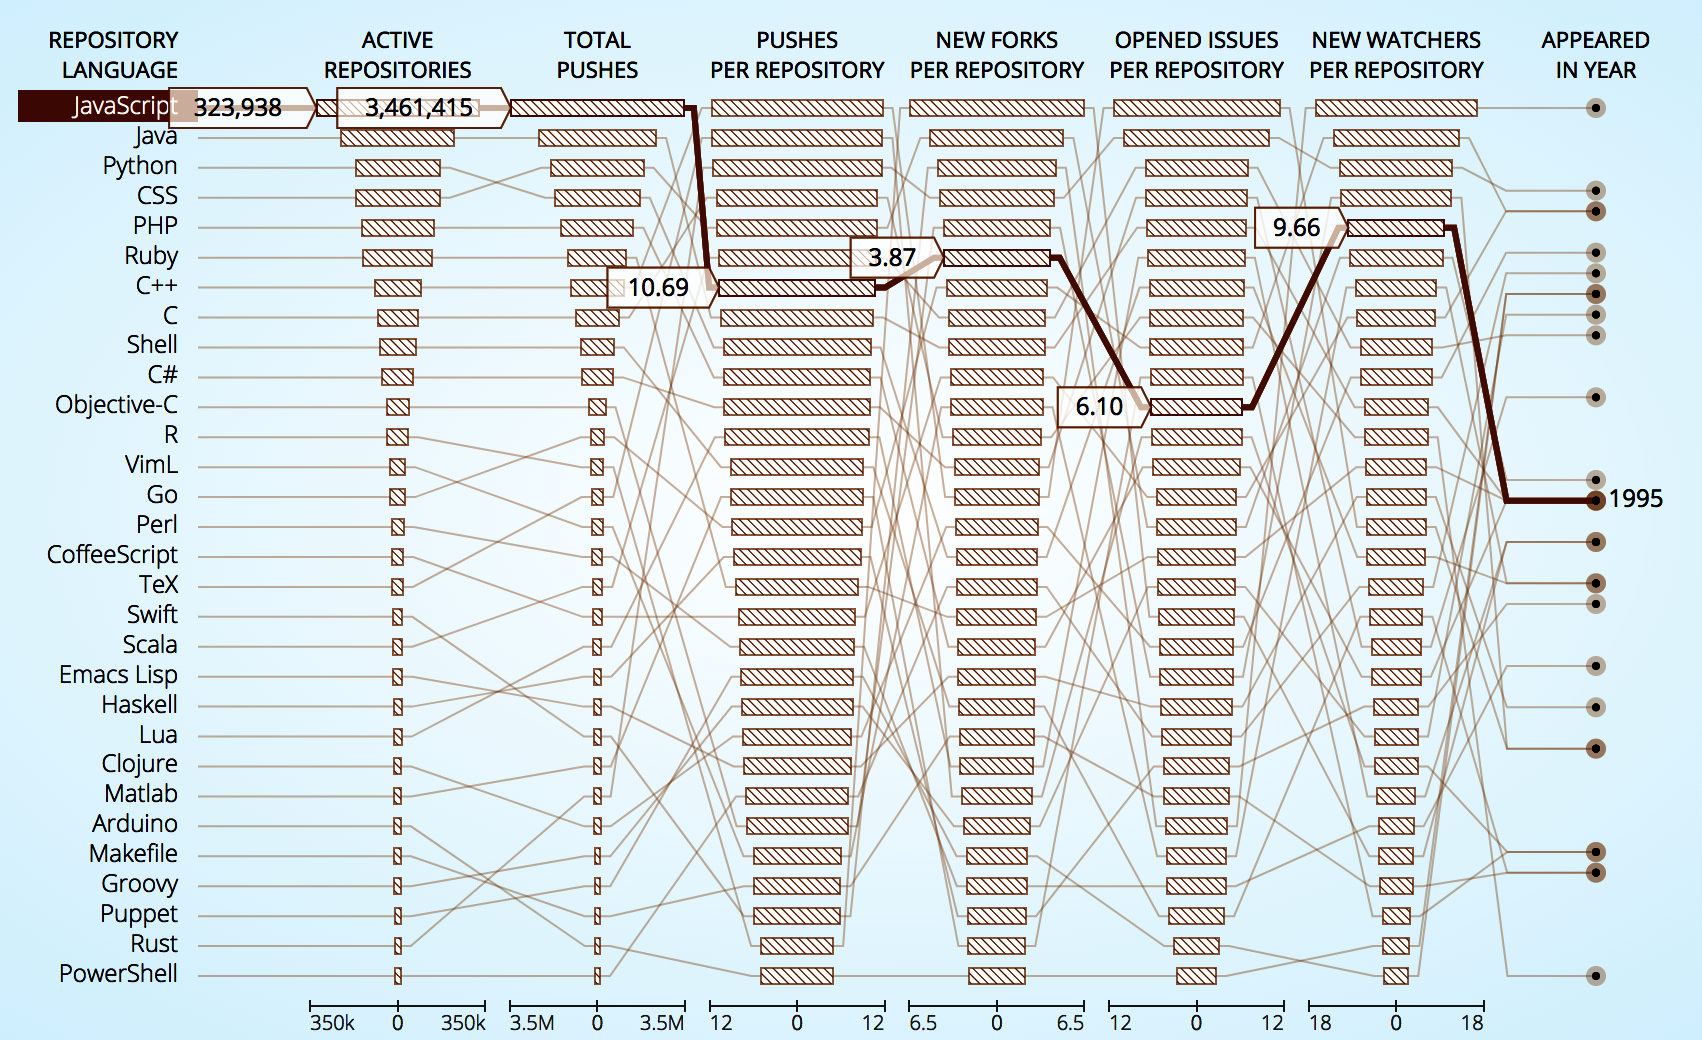
\includegraphics[width=\linewidth]{bilder/grundlagen/jsUsage.png}
	\caption{Numbers of Github repositories using JavaScript 2014 \cite{GitHut}} 
	\label{fig:JSgithub}
\end{figure}

\section{JavaScript}
Today JavaScript is one of the most used programming languages world wide.

JavaScript first appeared in 1995. Originally developed at Netscape
by Brendan Eich under the name of "LiveScript" it had a simple purpose, namely to dynamically manipulate the HTML Document Object Model (DOM) tree in the browser. 
 
At about the same time a company called Sun worked on a programming
language for embedded and mobile devices called Java.   
As Java became increasingly popular,
Netscape considered it a good marketing move to rename its
LiveScript to JavaScript, even though there was little technological
similarity between these two languages.
    
Java is a regular, static, and highly typed programming language.
It runs on a virtual machine and needs to be compiled, whereas the
single threaded JavaScript only runs in a browser and is a script
language. 
  
Both languages have in common a C related syntax and exhibit some 
similarities with regard to naming conventions. While Java is a true
object oriented language, JavaScript has incorporated elements
supporting object oriented programming only over time \cite{Bewersdorff2018ObjektorientierteProgrammierung}. 
  
The JavaScript community considers this language superior for web development. Jeff Attwood, the co-founder of 
the  computer programming question-and-answer website Stack Overflow and Stack Exchange, even said: 
"Any application that can be written in JavaScript, will eventually be written in JavaScript" \cite{Louis2018Java}.
 
\subsection{JavaScript distributed architectures}

Most modern web designs rely on a three-tier architecture (Fig. 
\ref{fig:TT}). The bottom tier is usually a database system, responsible for storing and retrieving data.\index{ three-tier architecture} Typical 
technologies employed here are relational database management systems (RDBMS) and, more recently noSQL database systems like key value stores \cite{GOLL}.  

The second tier is usually responsible for executing the application logic.
The technological base for this layer is Java, .NET, and more recently Node.js.
 
The top most tier is typically responsible for the user interface, but can also contain application logic.
The most widely used technology nowadays is a web browser with JavaScript programs. 

\begin{figure}[H]
	\centering
	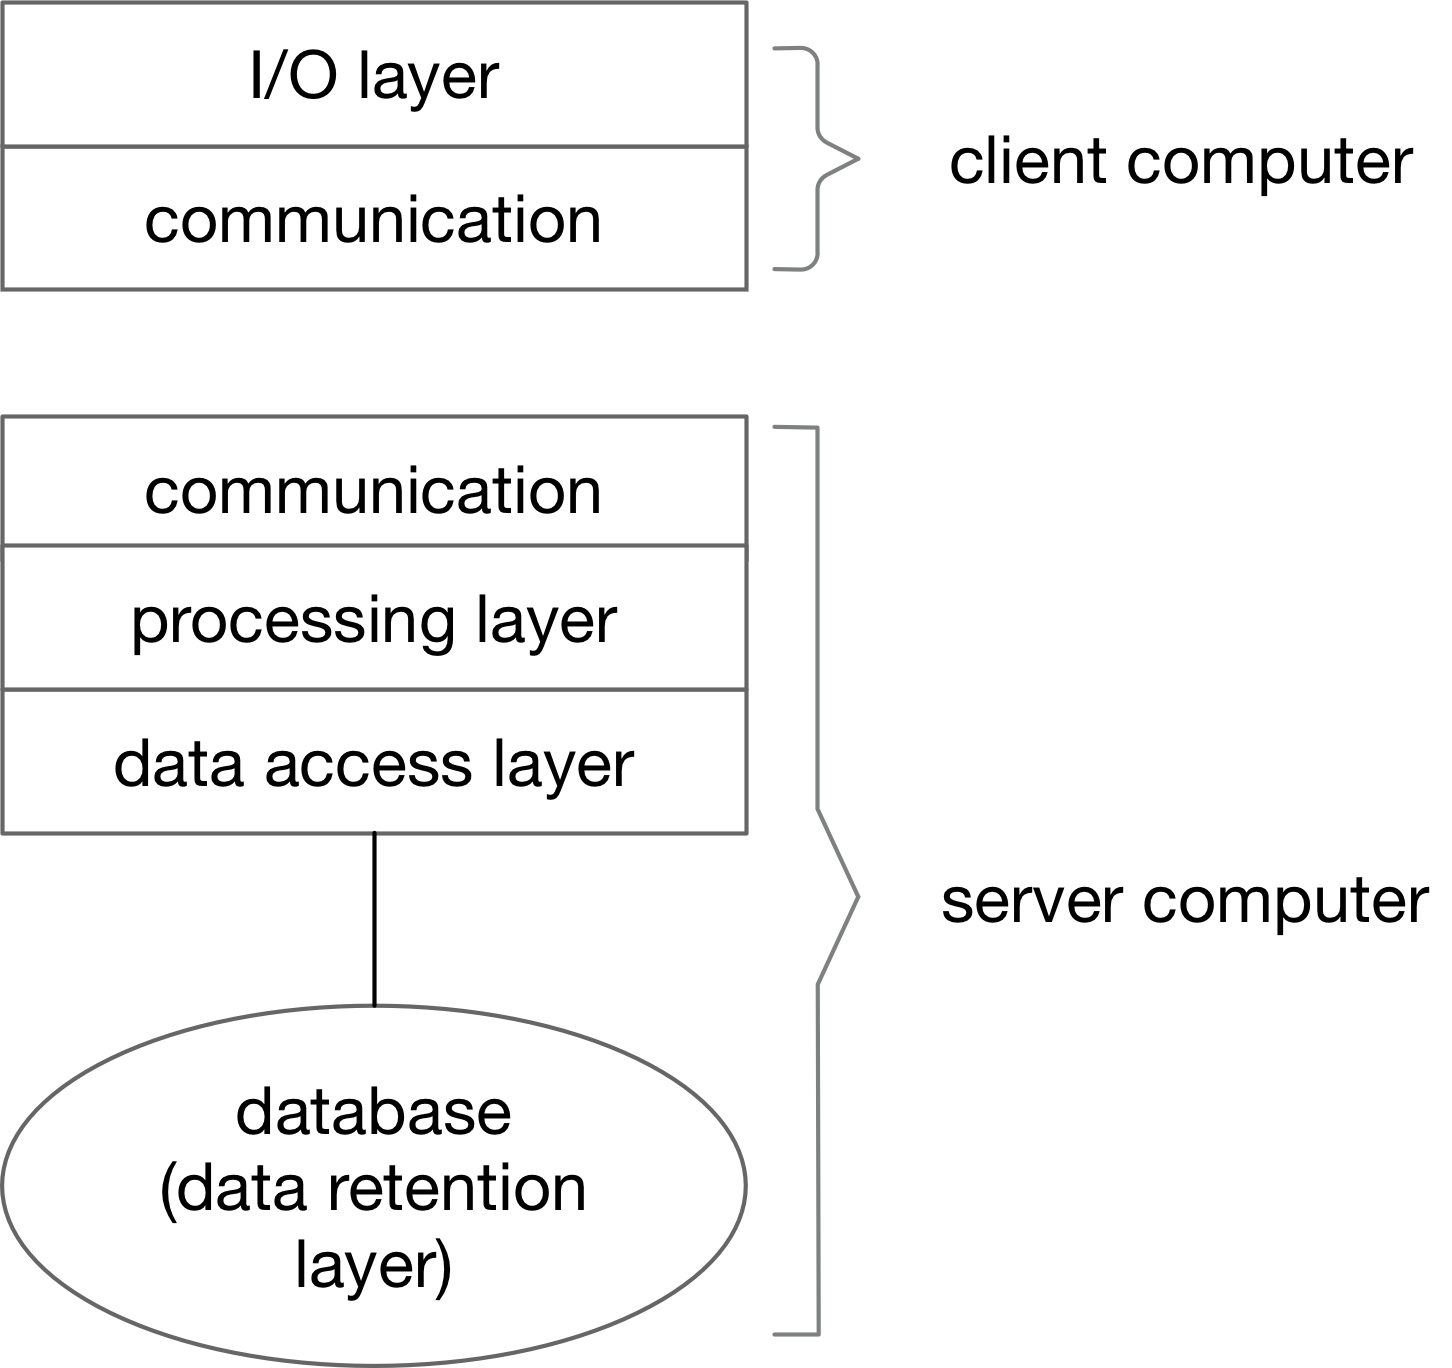
\includegraphics[width=0.5\linewidth]{bilder/grundlagen/Three-Tier.png}
	\caption{Three-Tier architecture \cite{GOLL}}
	\label{fig:TT}
\end{figure}

The three tier architecture requires a wide spectrum of technological know-how:
Know\-ledge about database management systems which is a discipline on its own,
then deep knowledge of the Java or  .NET ecosystem, and knowledge about HTML, 
cascaded style sheets, JavaScript 
and possibly JavaScript frameworks used for the design of the user interface.

To reduce the amount of programming languages to be used some people have advocated 
JavaScript also as a server side language. This has become  popular with the Node.js 
framework which permits JavaScript developers to employ their programming language 
skills on the client side as well as on the server side. 

On the account of type safety, this approach fosters rapid application development.
Using a single language on both sides adds the chance of sharing modules,
thus further reducing development time (see Figs. \ref{fig:DS1} and  \ref{fig:DS2}).
This novel approach even affects the job market. Iin the past front-end and back-end developers 
had required different 
skills. This has changed now and people can do full-stack web development with just 
good JavaScript knowledge. 
 

\begin{figure}[H]
	\centering
	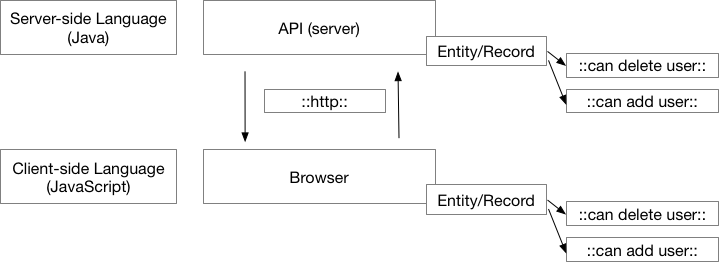
\includegraphics[width=0.8\linewidth]{bilder/grundlagen/Entity1.png}
	\caption{Duplication of functionality due to heterogeneous programming languages}
	\label{fig:DS1}
\end{figure}

\begin{figure}[H]
	\centering
	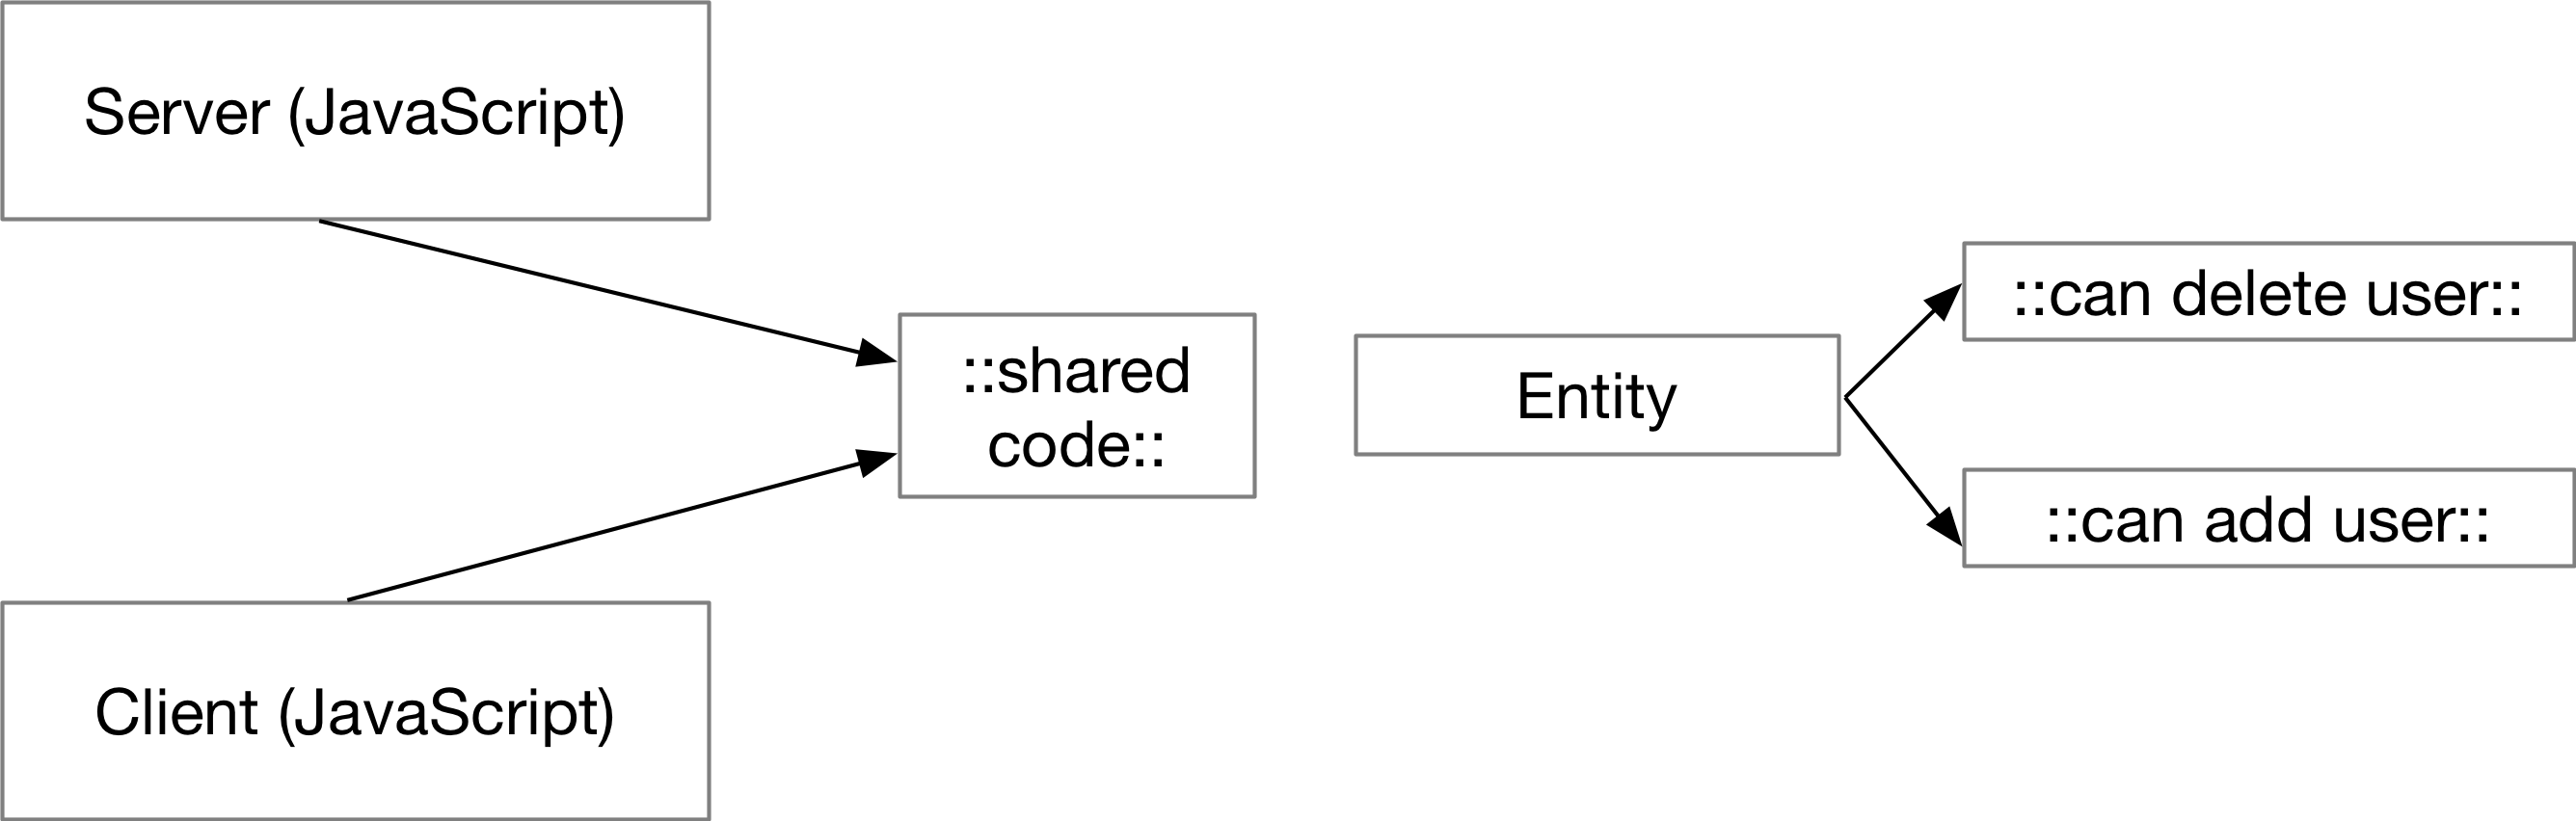
\includegraphics[width=0.8\linewidth]{bilder/grundlagen/Entity2.png}
	\caption{Reuse of shared modules due to a single language approach}
	\label{fig:DS2}
\end{figure}


\subsection{Multi-Platform support}


It is expensive to develop an application for a number of platforms like Android or iOS for tablets and Windows,
Linux or MacOs for desktop computers. Creating applications for any of these platforms
requires large amounts of platform specific code while little can be shared.
Java has provided a way out of this dilemma with the exception of the popular iOS. \index{iOS}
Apple does not allow Java to run
on their mobile devices.

There exist other cross-platform frameworks like QT. However, they require people to program in C++
which is not the most efficient way to create user interfaces anymore.


With JavaScript developers can take advantage of modern frameworks like React Native or Electron, which make it possible to almost completely code in JavaScript. 

The JavaScript communicates with native components that might be written in Java on
Android, in Objective C on iOS, in CSharp on Windows and so on. A so called "bridge"
(see Fig. \ref{fig:BP}) forwards calls from JavaScript to native components and returns
responses back to the JavaScript part. This facilitates user interfaces to 
have a native look and feel even though they are written in JavaScript \cite{Purewal2014LearningWeb}.

\begin{figure}[H]
	\centering
	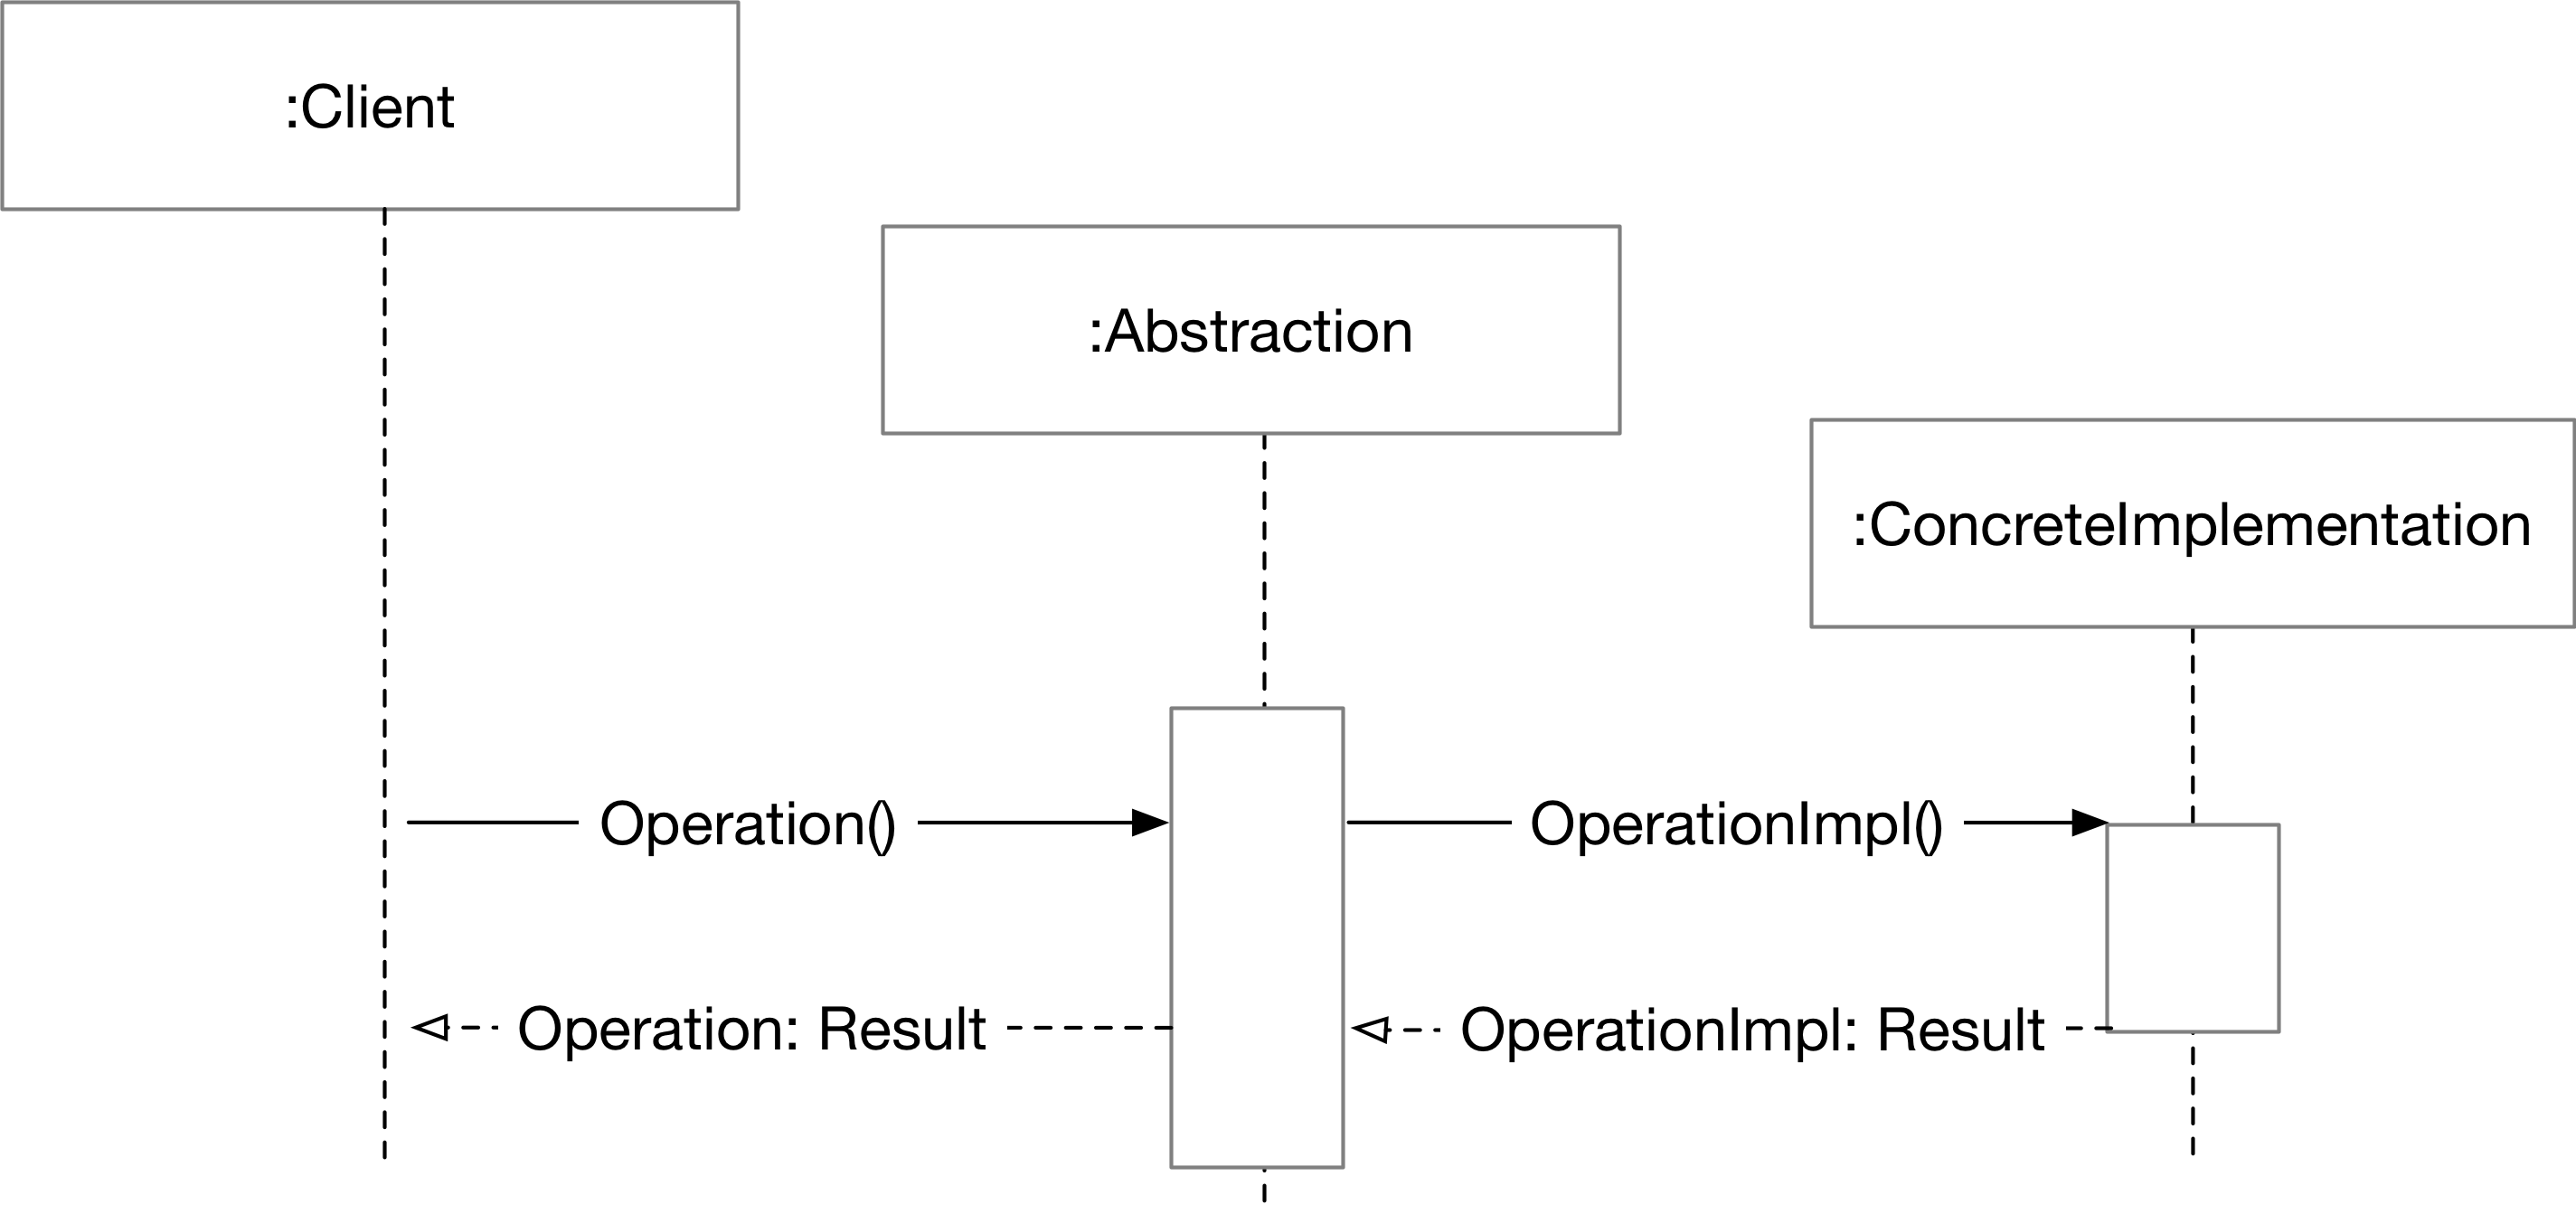
\includegraphics[width=1.0\linewidth]{bilder/grundlagen/BridgePattern.png}
	\caption{Bridge pattern \cite{GOLL}}
	\label{fig:BP}
\end{figure}


\subsection{Single threading and concurrency}

JavaScript is a single threaded programming language with some extension for asynchronous processing.
A JavaScript program may never have an infinite loop, regardless at which level.
This is due to the fact how JavaScript handles concurrency. JavaScript was developed to manipulate the DOM. 
The DOM is a singular structure and it is easily conceivable that changing it from different threads would result in a big mess.
Thus it made no sense to have JavaScript support concurrency.

On the other hand the browser had to interact with remote servers 
which could lead to large delays until a response would have been received.
Blocking the single JavaScript thread with such calls would have lead to
a rather poor user experience, basically blocking 
any user interaction while the browser was waiting for
the servers response.

The designers of JavaScript therefore provided a way to execute outside asynchronous calls
with so called "callbacks".  Every time a function is called in JavaScript, it is put on a call stack.  
Once the function returns 
the result is popped from the stack.  Each function on the stack is executed purely synchronously 
one after the other (see Fig. \ref{fig:CS}).

\begin{figure}[H]
	\centering
	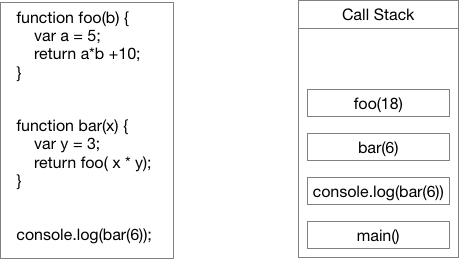
\includegraphics[scale=0.6]{bilder/grundlagen/CallStack.png}
	\caption{Call Stack}
	\label{fig:CS}
\end{figure}

In order to execute code concurrently, JavaScript needs to call the Web API provided by the browser. The web browser runs on a multi threaded operating system so it fully supports concurrency. 

The Web API is called with the function that needs to be executed,  and a callback function.
The callback function is called by the asynchronous function when it finishes execution. \index{asynchronous function}
It is mandatory to provide a callback with each asynchronous function call.

Once the thread executing the asynchronous function is finished it passes the callback to the so 
called "callback queue".
The callback queue is a simple list containing all callbacks waiting for execution.

An event loop continuously checks if the call stack is empty. As soon as that is the case the first 
callback function from the callback queue is placed on the callstack and executed synchronously. 
This decoupling of the caller from the response allows JavaScript to do other things while waiting 
for asynchronous operations to complete and their callbacks to fire (see Fig. \ref{fig:CC}).


\begin{figure}[H]
	\centering
	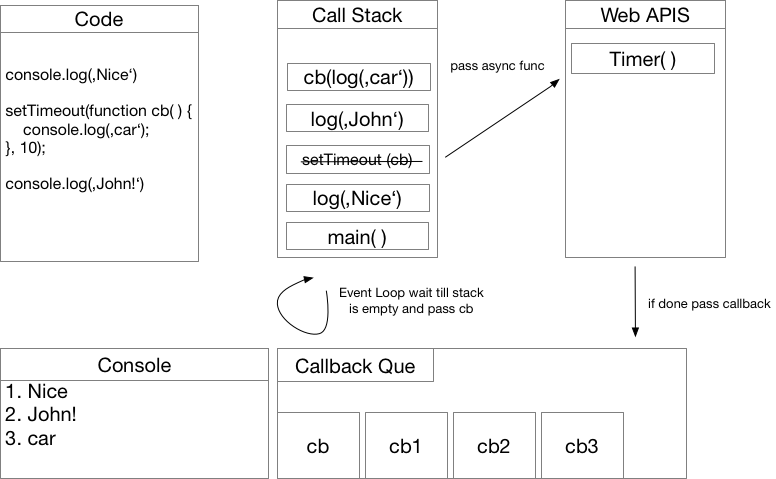
\includegraphics[width=1.0\linewidth]{bilder/grundlagen/Concurrency.png}
	\caption{Concurrency in JavaScript}
	\label{fig:CC}
\end{figure}

\subsection{Functional programming paradigm}

JavaScript is a functional programming language, that is it is possible to 
pass functions as parameters and to return
functions as results. In the functional programming paradigm the return value of a function shall not depend on global variables or state variables, it shall purely depend on its input arguments (see Fig. \ref{fig:FP})\cite{Steyer2014JavaScript}. \index{functional programming}

In the latest releases of the JavaScript standard provisions have been made to better support the object
oriented paradigm.

\begin{figure}[H]
	\centering
	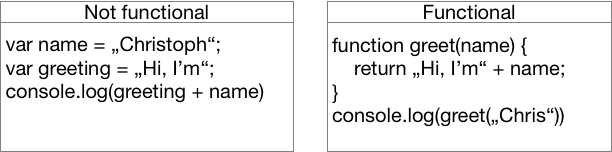
\includegraphics[scale=0.6]{bilder/grundlagen/fp.png}
	\caption{Imperative and functional programming}
	\label{fig:FP}
\end{figure}

In JavaScript it is possible to define functions as part of higher-order functions  \ref{fig:HF}. 

\begin{figure}[H]
	\centering
	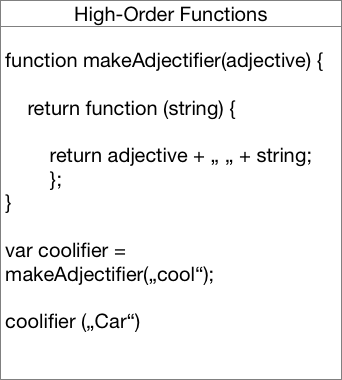
\includegraphics[scale=0.6]{bilder/grundlagen/fp1.png}
	\caption{High-order functions}
	\label{fig:HF}
\end{figure}

\section{Software patterns for web-development}

\subsection{The classic model view controller model}

For a long time it was best practice to use the model view controller (MVC) architectural 
pattern for implementing user interfaces.\index{model view controller}
In this pattern, the model stores the data 
presented in one or more views. In simple systems the model may contain some
 business logic (see Fig \ref{fig:MVC}).

The controller controls the model and view state, based on user input.
For example it activates or deactivates buttons.
 It also transforms events caused by user actions into method calls of the model 
\cite{GOLL}. 
 
The view serves to present model data to the user. There can be many views on the 
same model data. In case of a model data change all views are updated. 
Beside presenting model data the view also provides interactive elements.

The model shall be independent of views and controllers. In case the model changes, 
the controller may inform the views (passive model). With the alternative active model 
implementation, the model informs the views of any change.

\begin{figure}[H]
	\centering
	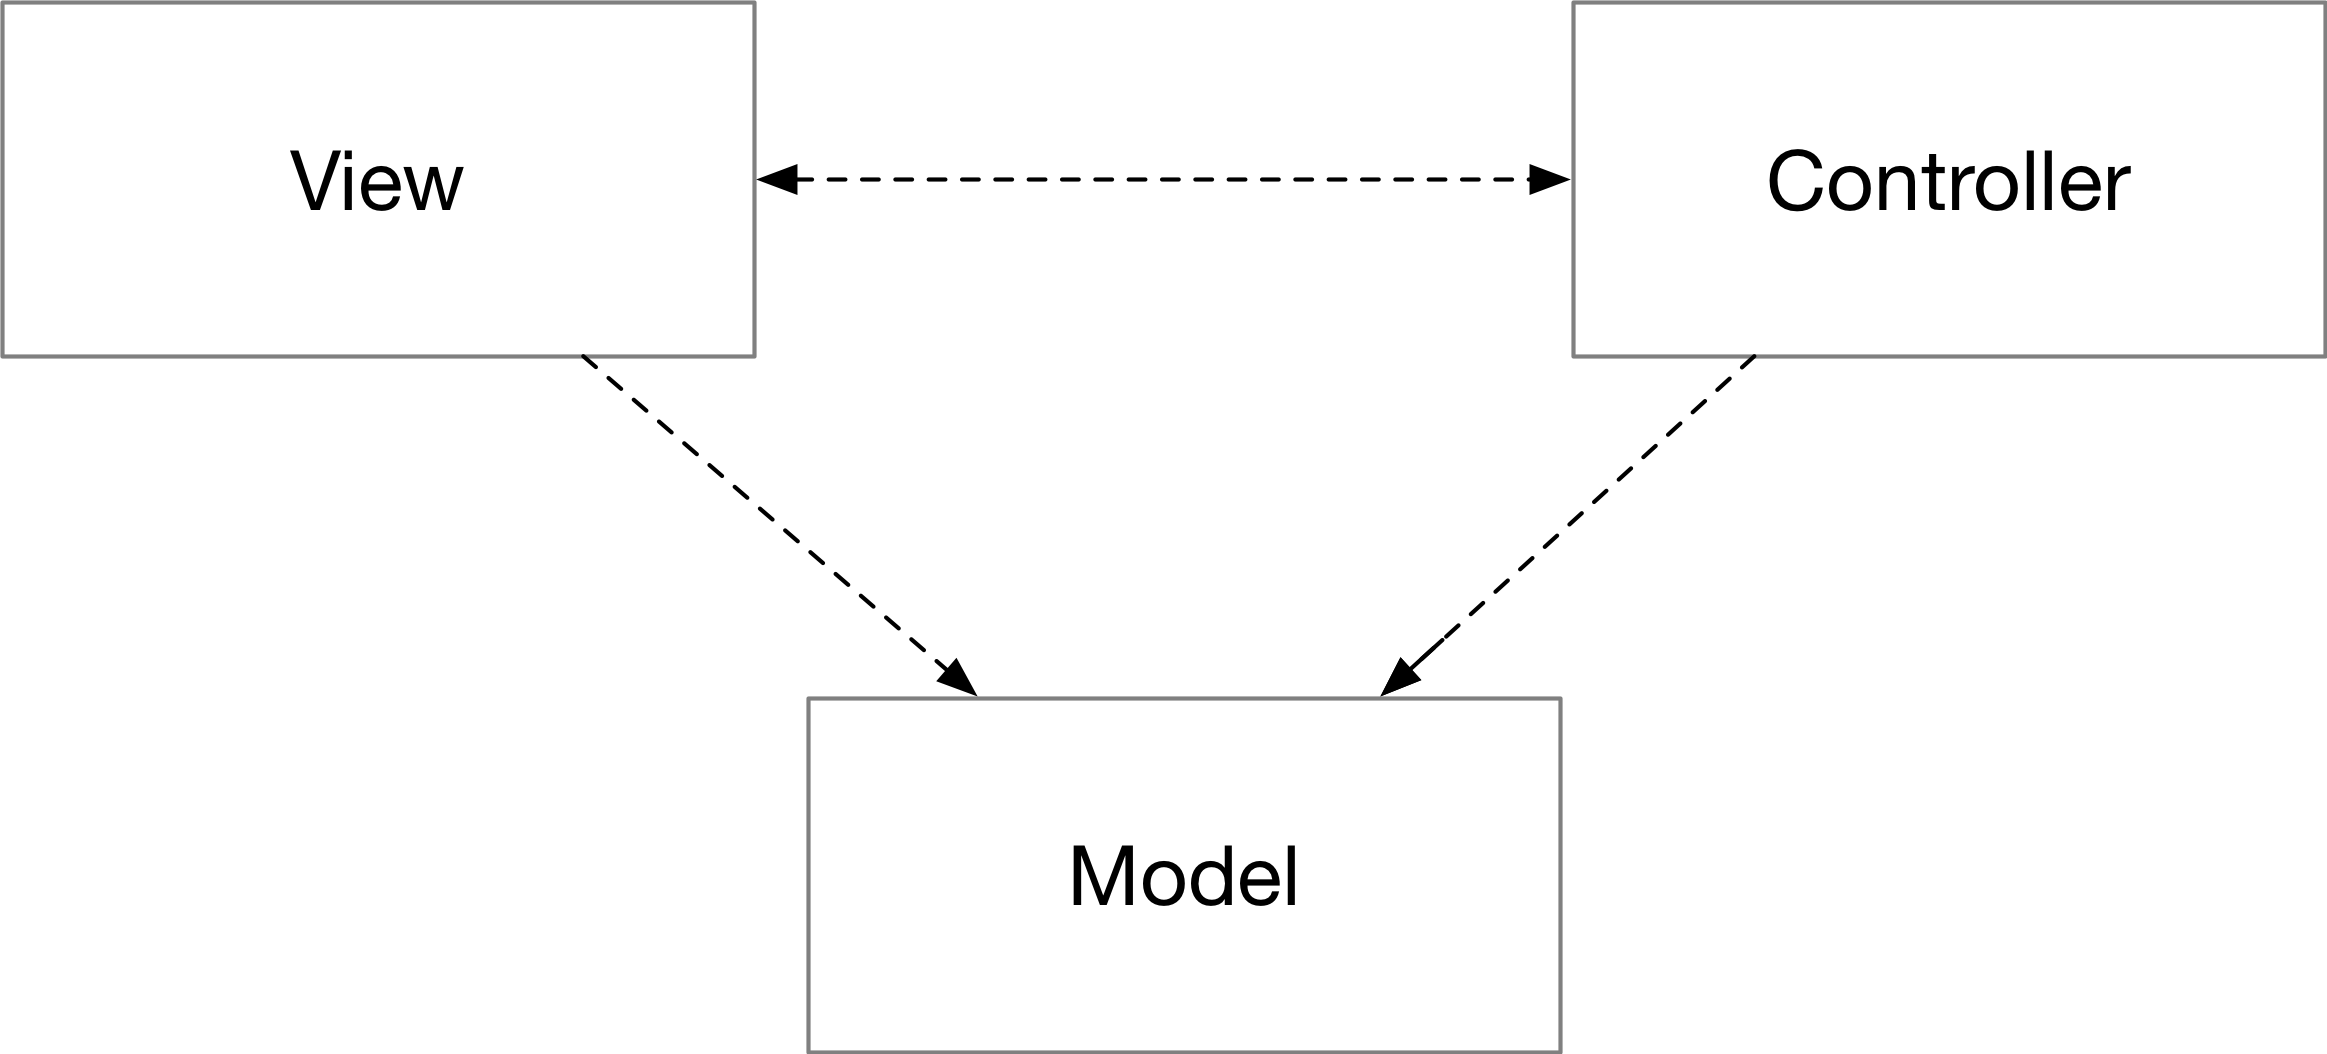
\includegraphics[scale=0.6]{bilder/grundlagen/MVC.png}
	\caption{MVC  software architecture  \cite{GOLL}}
	\label{fig:MVC}
\end{figure}

The so called principle "separation of concerns" makes it easier to split work and thereby 
makes it easier to maintain code.
A drawback is the increased number of classes and larger complexity.
For example,  changes in the model or the controller affect the whole entity. 
The bidirectional communication in the MVC structure makes it hard to debug.
Changing one entity has a cascading effect across the codebase.

The React framework tries to keep the benefits of the MVC pattern while at the same time 
avoiding some of its disadvantages. To that end it employs a different architecture called
Flux which shall be explained below.

\subsection{Flux}

\subsubsection{Structure and data flow}
The Flux architecture consists of actions, dispatchers, stores and views. In Flux data flows in a single direction.
The unidirectional data flow is central to the Flux concept (see Fig. \ref{fig:FLUX}).
Dispatcher, stores and views are independent nodes with different inputs and outputs. The actions simply consist of objects with the new data. The following sections are inspired by the official Flux guide \cite{Flux}. \index{Flux}

\begin{figure}[H]
	\centering
	
\includegraphics[scale=0.5]{bilder/grundlagen/UniDirection.png}
	\caption{Flux software architecture \cite{Flux}}
	\label{fig:FLUX}
\end{figure}

The dispatcher takes care of handling all actions and forwards them to the proper store.
The store holds the data and actions to change this data.
Once data was changed the store alerts all views that are affected by this data change, causing a re-rendering (see Fig. \ref{fig:FA}).

It is also possible that a view generates an action. This happens mainly through user interaction. This action is also passed to the dispatcher. \index{dispatcher}

\begin{figure}[H]
	\centering
	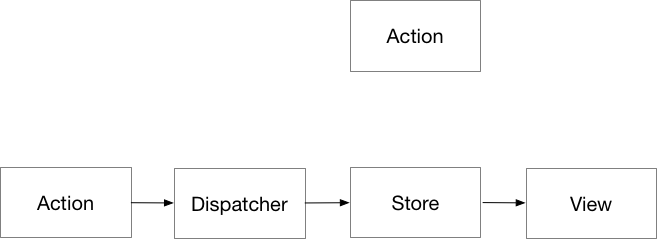
\includegraphics[scale=0.5]{bilder/grundlagen/uniDirection2.png}
	\caption{Flux with view action \cite{Flux}}
	\label{fig:FA}
\end{figure}

\subsubsection{Stores}
Stores contain the application state and the logic. 
Their role is similar to that of the model in the MVC,
but they can contain the state of several objects. 

Stores typically comprise the states of a domain within the application.
Stores register with the dispatcher with a callback function.
The callback has an action as a parameter.
A switch case based on the action type determines which method within the store should be executed.

In this way a store is updated by an action. As soon as the store is updated,
it reports that a state has changed so that all views can get the new state and update themselves.

\subsubsection{Dispatchers}
In the core of Flux lies the dispatcher. It is responsible for the control of the data flow within the application. In principle, it consists of a list of callbacks into the various stores.  It serves only to distribute the actions to the various stores. Each store registers itself with a dispatcher providing a callback . The dispatcher can also consider dependencies between different stores and control the order of the callbacks.

\subsubsection{Views and controller-views}

In React all views are composable and freely re-renderable. 
At the top of the view hierarchy there is a hidden view that listens to events that are sent by the store.
It is called a controller-view. 
The controller-view fetches the data from the store and passes it down to all descendants,
causing a re-rendering. Often the entire state of a store is passed down a chain of views allowing each descendant to take what it needs.

\subsubsection{Actions}

The dispatcher provides a dispatch method that has an action as a parameter. Actions can either be sent directly to the dispatcher or created via a creator function and sent to the dispatcher. The creation of an action usually takes place in the event handler of a view, for example due to a user interaction or a browser event.


\subsubsection{Conclusion}
The Flux architecture improves data consistency. 
The unidirectional data flow makes  applications based on Flux much easier to debug, 
since one can always follow easily the flow of actions. 
Furthermore, having the state and all logic updating the state in one place
it is also possible to do more meaningful unit tests.

\section{React and Flux}

The key framework used in this project is React, a  JavaScript library for developing user interfaces \cite{React}.

Back in 2011 Facebook noticed that it was getting hard to maintain
their application and to run it flawlessly, due to the  growing number of features.
Many people were hired and the team size expanded significantly.
With the growing team size it took longer to publish urgent updates.
Too many people were involved and concerns could not be separated in a satisfying manner.

A Facebook engineer called Jordan Walke decided to change that.
In the same year he created FlaxJs, a first prototype of React. 
Jordan was allowed to keep on working and created React in 2012. 

A short time later Instagram was bought by Facebook and both
companies agreed on using React as the new core technology for user experience.
 Further they agreed on making React publicly available. 

In early 2013 at JS ConfUS, React became an open source project. Facebook CEO Mark Zuckerberg, speaking on this conference said:  "Our biggest mistake was betting too much on HTML5". He promised to provide better experiences with React.

Currently React is getting increasingly popular. A trend analysis by Google shows that 
React is the leading modern user interface JavaScript framework (see Fig. \ref{fig:React}).

\begin{figure}[H]
	\centering
	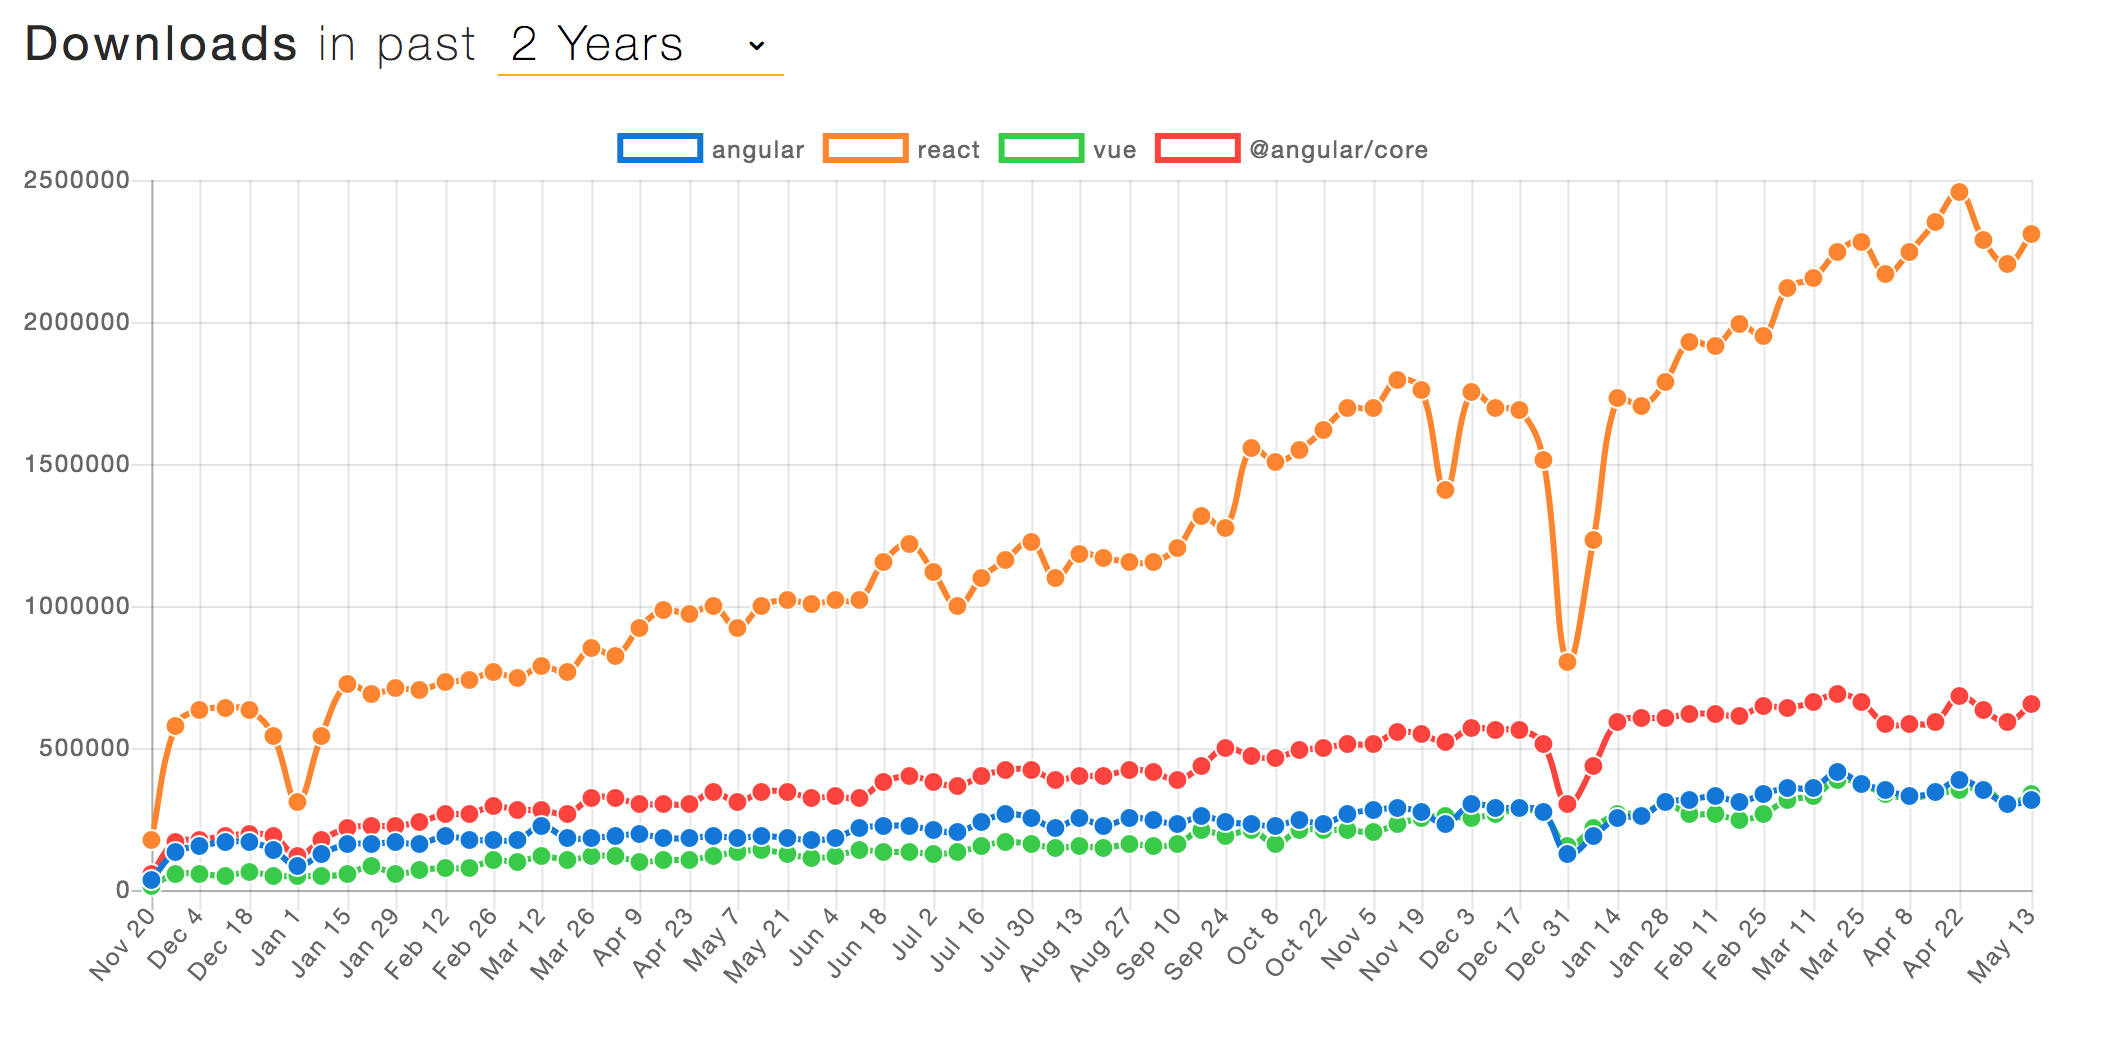
\includegraphics[scale=0.4]{bilder/grundlagen/ReactDownloads.png}
	\caption{Downloaded npm packages \cite{NPM}}
	\label{fig:React}
\end{figure}

This section is about analyzing how React is implementing the Flux software architecture. 
React is based on encapsulated components that manage their own state.
An application consists of nested components, somehow similar to the tree structure of an HTML DOM.

Components are written in JavaScript, so data can easily be passed through the application.
Any element that needs to be rendered is still written in HTML and parsed by React.
Each component has its own controllers.

In React, there are no HTML files decorated with special tags
but rather the HTML is generated from within JavaScript code.
Every component is fully standalone and testable on its own.
This makes React scalable and easy to test. There are no cascading dependencies.
Every time the state of a component changes,
the render function is called and the HTML is re-rendered with the changed data.
Components can be nested, for example a board game that consists of squares (see Fig. \ref{fig:Grid}).

\lstinputlisting[caption=Nested square component]{code/grundlagen/Component.js}

Each square is a component and part of the whole board game application.
There shall be a value assigned to the squares. Values are passed down to lower components via the 
"props" variable. 

\lstinputlisting[caption= Passing down variables with props]{code/grundlagen/ComponentWithProps.js}

\begin{figure}[H]
	\centering
	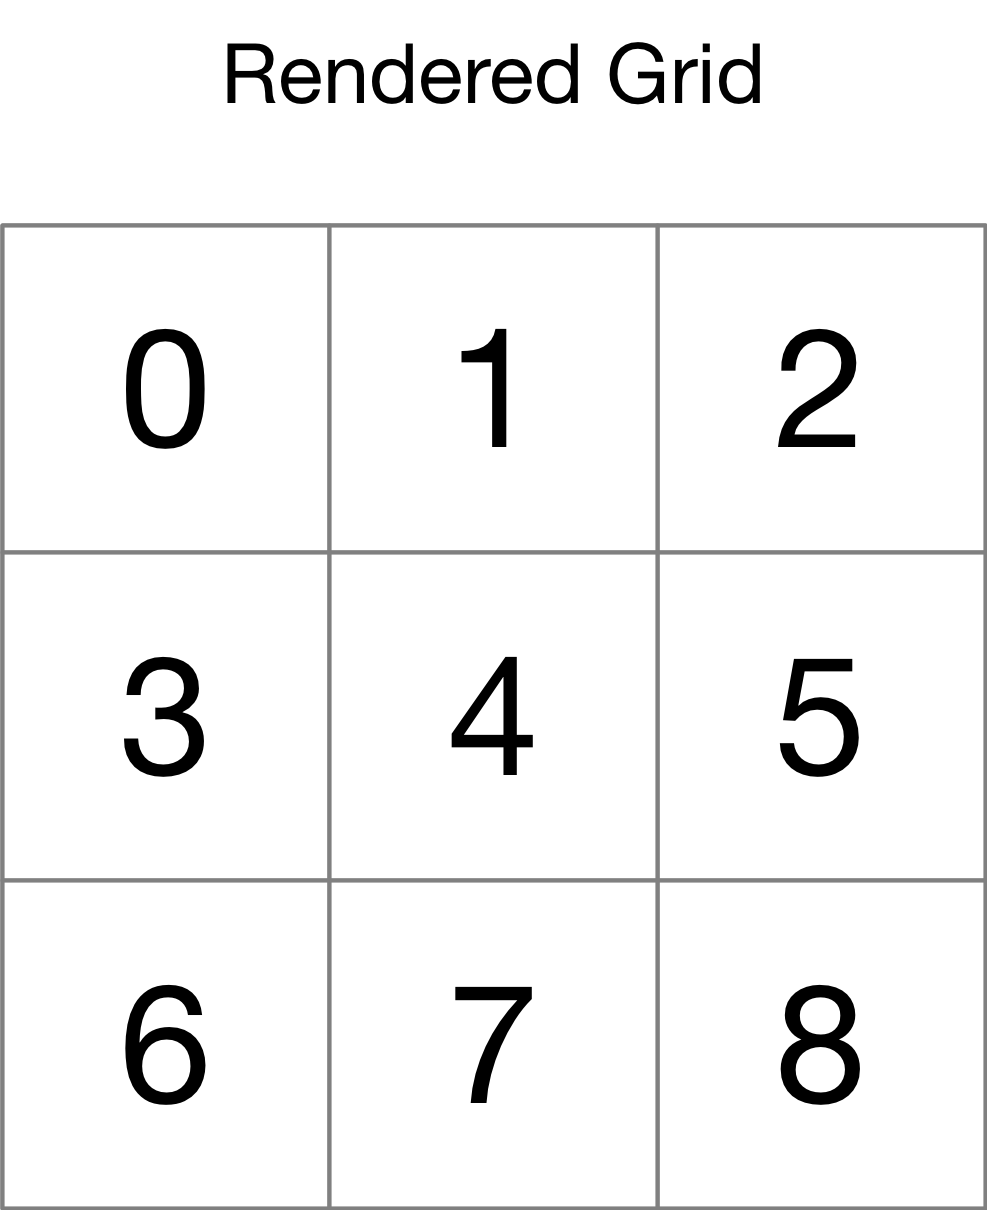
\includegraphics[width=0.3\linewidth]{bilder/grundlagen/GameGrid.png}
	\caption{Grid with numbers}
	\label{fig:Grid}
\end{figure}

Squares that have been clicked on shall show an 'X'. This value can be considered a local state.
It is definitely a private part of the square. First an initial state needs to be added.

\lstinputlisting[caption=Components with states]{code/grundlagen/ComponentWithState.js}

When \texttt{this.setState()} is called, an update is scheduled by React and the value is merged in the correct component state. Furthermore the component and all of its descendants are re-rendered. If a square was clicked it would now show an 'X' in the grid.

\subsection{Lifting state up}

Often data needs to be aggregated from multiple child components. 
Then it makes sense to lift all states up to a top-level component. 
The parent component  passes down the individual states to child components.

For example in a Tic Tac Toe game, to determine who has won 
the value of all square components would need to be checked. 
While that is technically feasible, a better approach is to save all states in the parent component.
The parent then checks the array in order to determine who has won.

The square component is no longer keeping its own state, it receives the value from its parent board. It informs the parent when it was clicked. Such components are called "controlled components" (see Fig. \ref{fig:TopLevel}).

\begin{figure}[H]
	\centering
	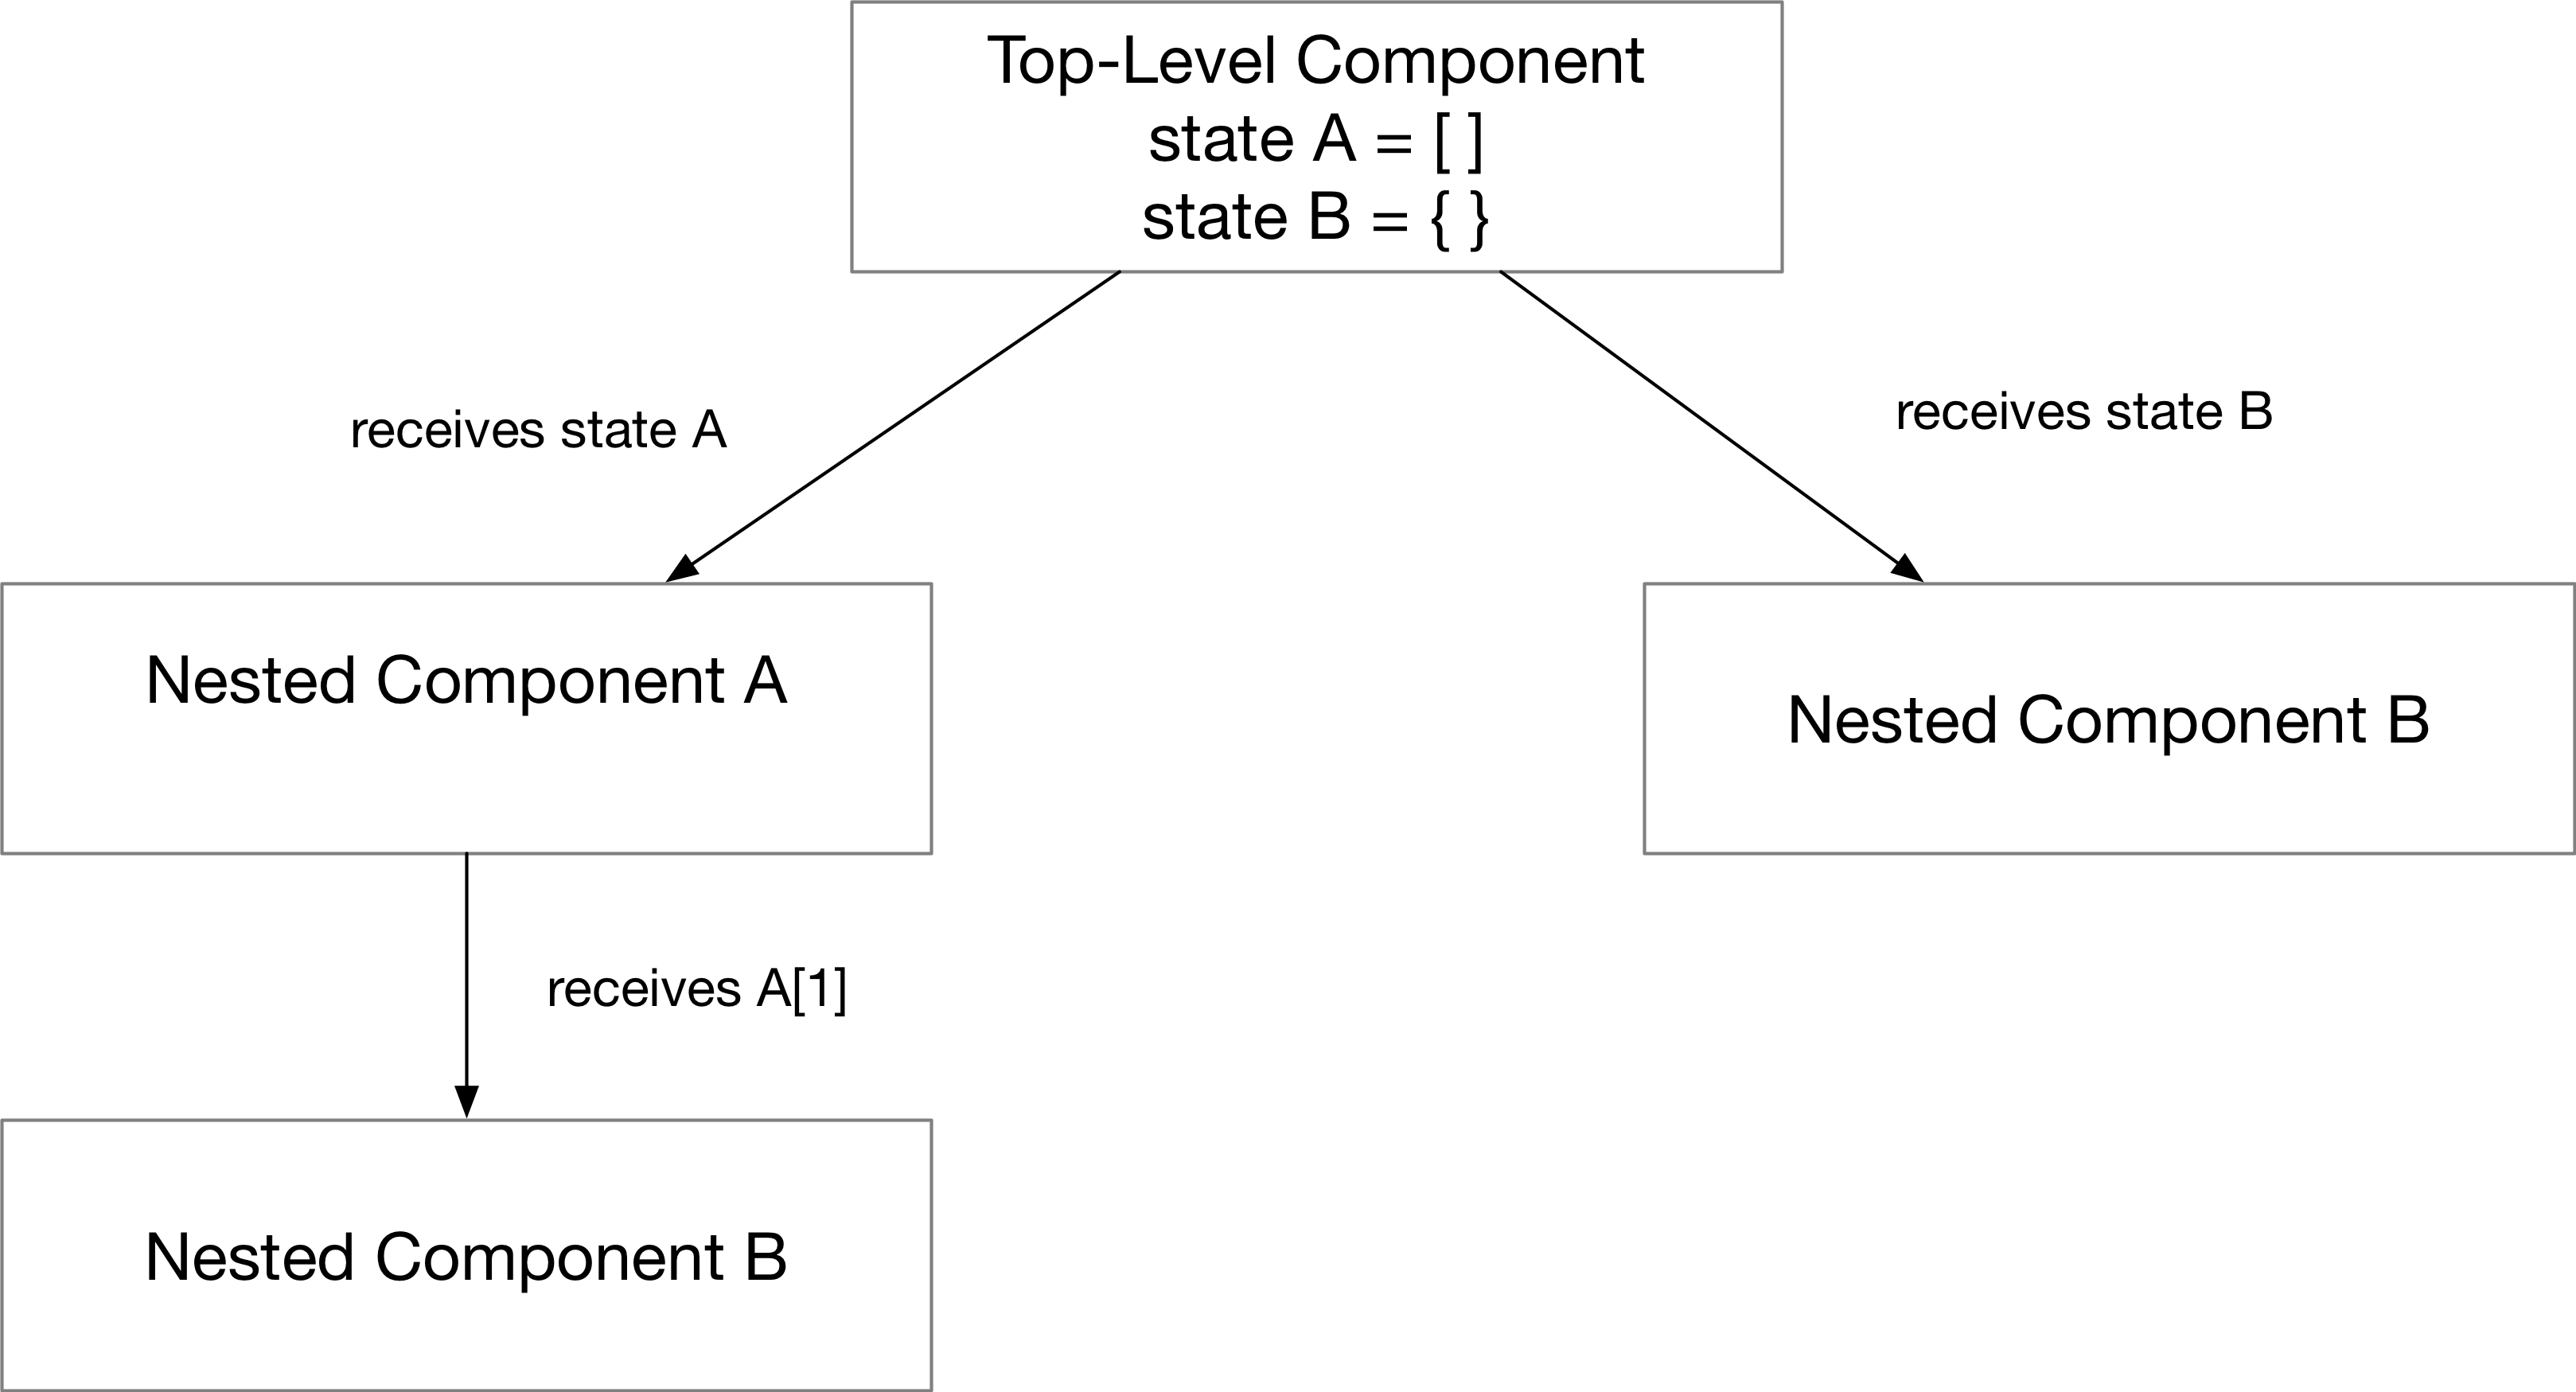
\includegraphics[width=1.0\linewidth]{bilder/grundlagen/topLevelComponent.png}
	\caption{Top-level component} 
	\label{fig:TopLevel}
\end{figure}


\subsection{Action- and dataflow}

Taking the last examples it is clear that data is only passed in one way, 
from the top-level component to a child component.
Another key principle is that actions are only passed up. 

For example if a nested component B is clicked or is triggered on a different event,  
some state B shall be changed in the top-level component. That is possible because 
all functions that change the data in the top-level component can be passed down 
to nested components via the \texttt{props} variable (see Fig. \ref{fig:DataFlow}).

\begin{figure}[H]
	\centering
	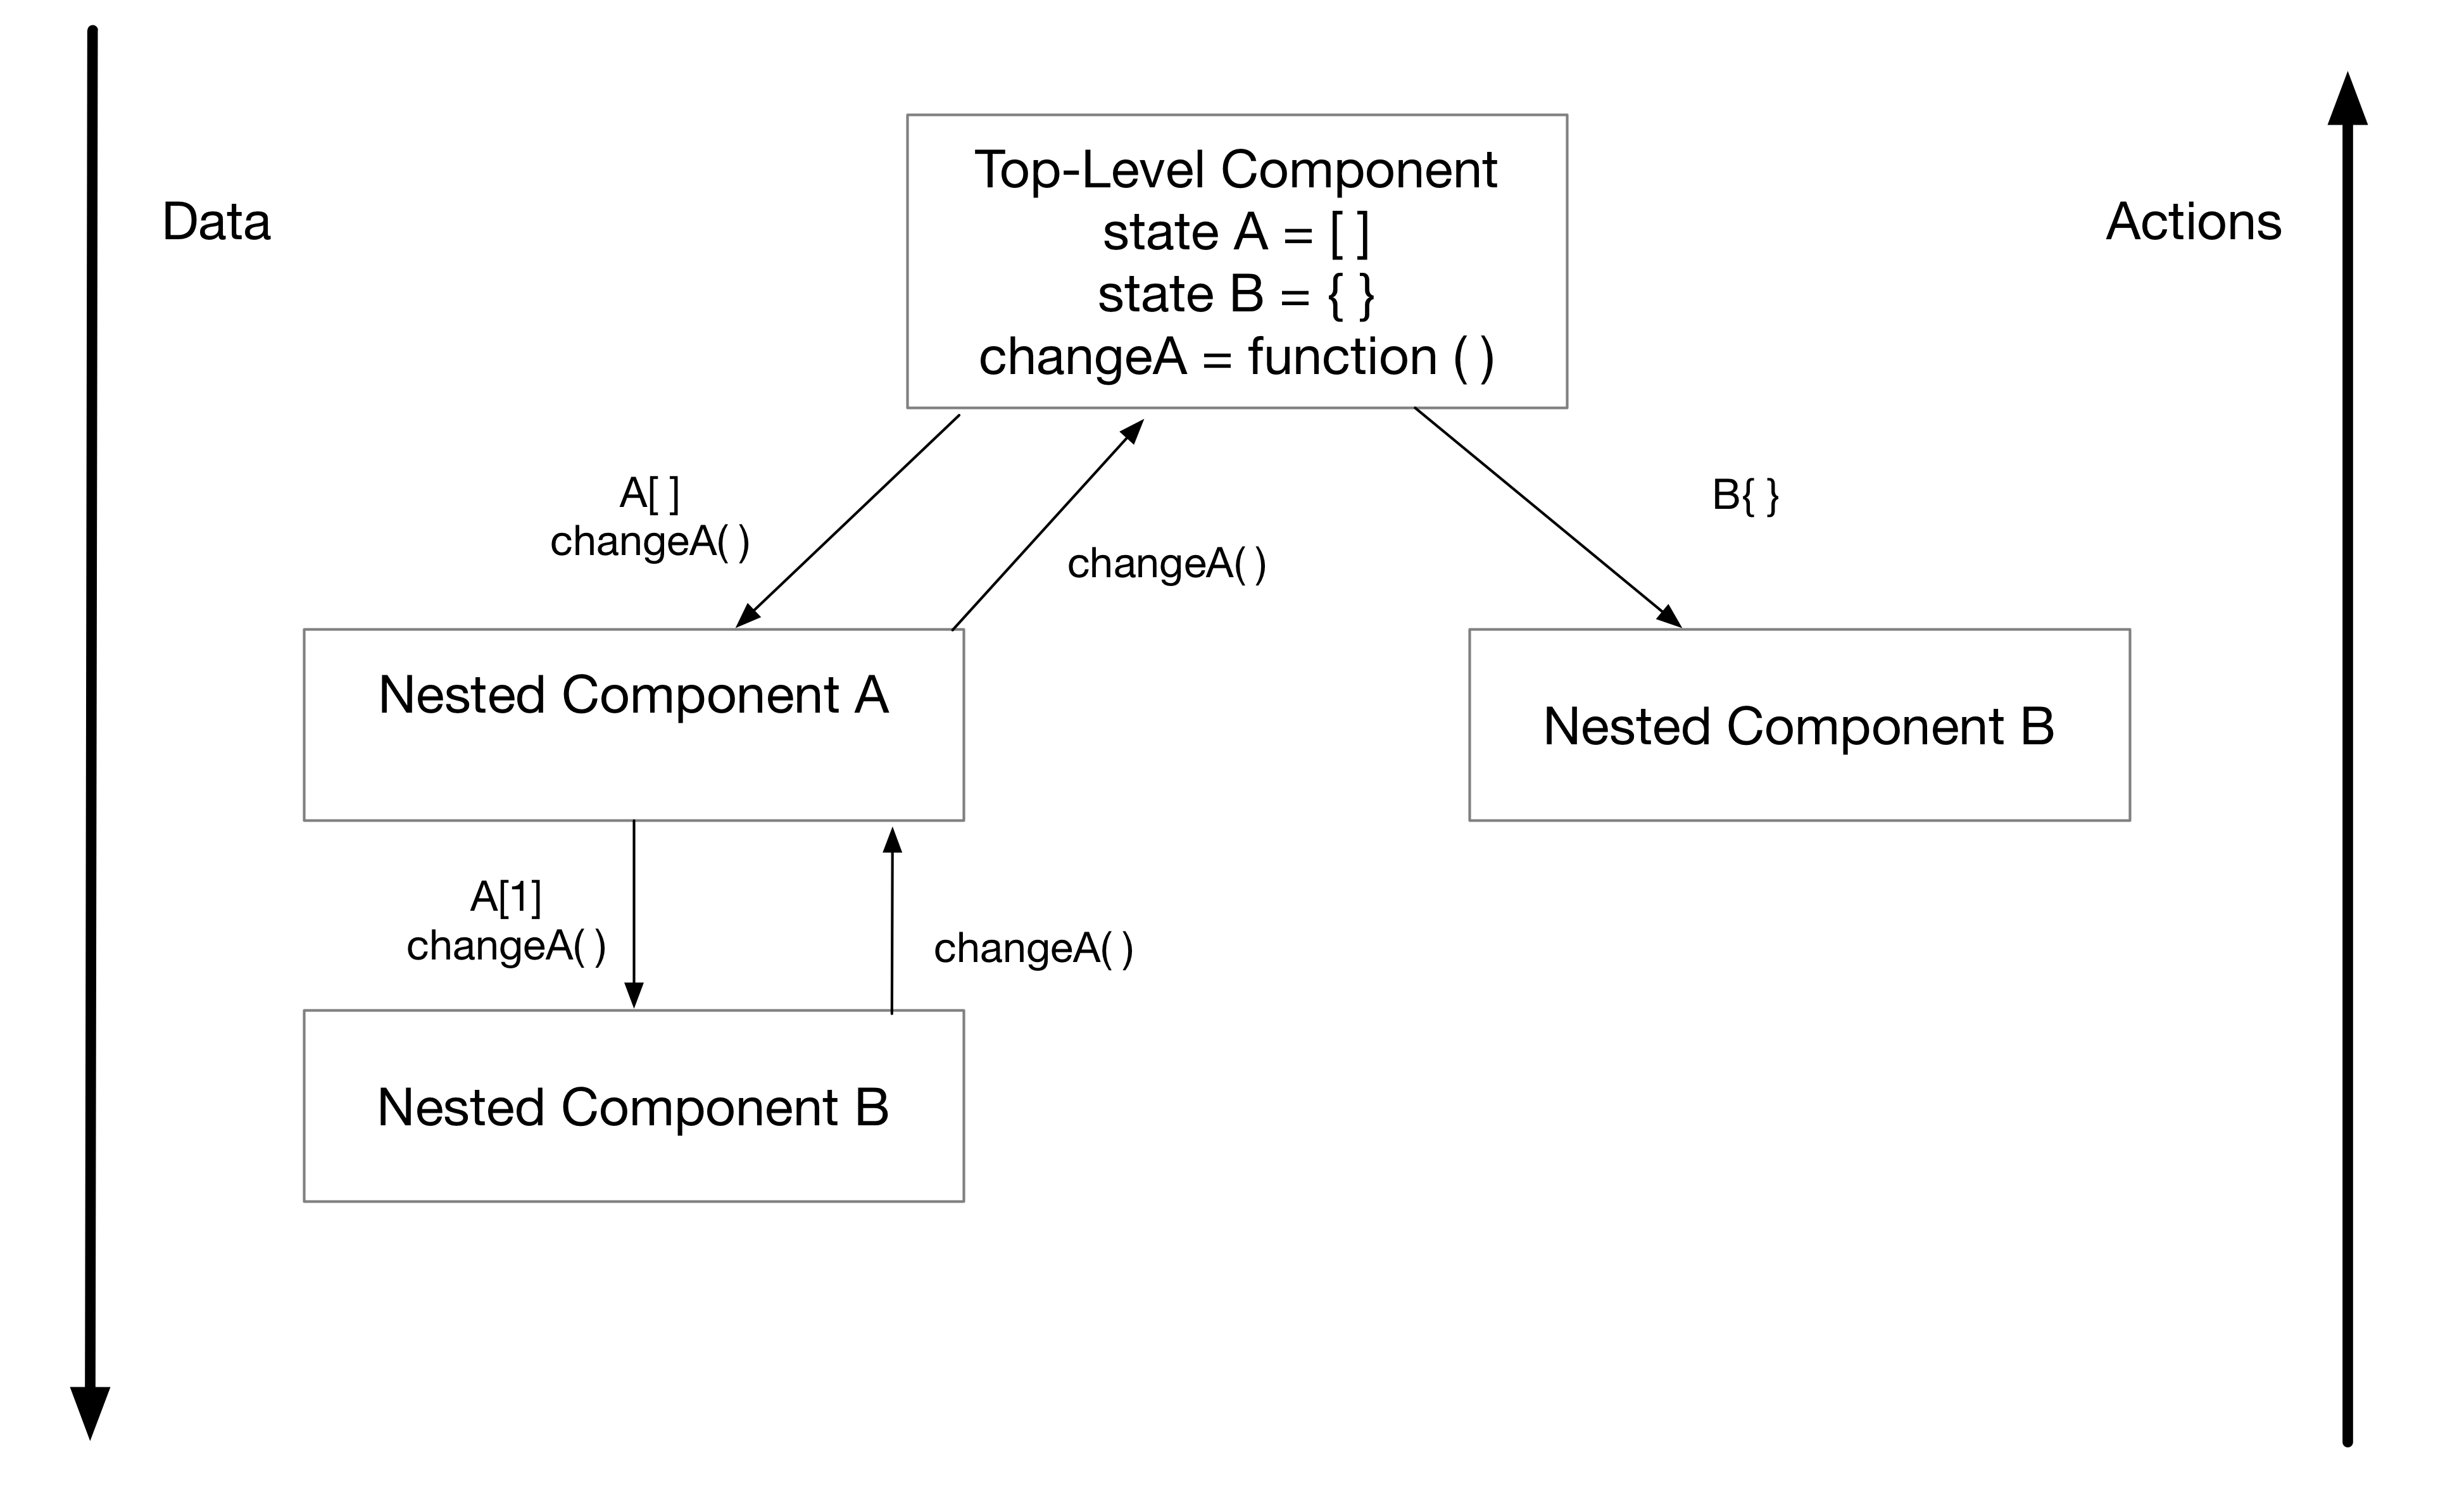
\includegraphics[width=1.0\linewidth]{bilder/grundlagen/dataFlow.png}
	\caption{Action- and dataflow}
	\label{fig:DataFlow}
\end{figure}


\subsection{High-order components}

As already known from the JavaScript introduction chapter
a high-level function can take another function as an argument.
Similar to that a high-order component is simply a high-order function
that takes a stateless component and returns the changed component. 
This makes it possible to add functionality to components on the fly. 

\lstinputlisting[caption=High-order component ]{code/grundlagen/hoc1.js}


\lstinputlisting[caption=Wrapped component]{code/grundlagen/hoc2.js}



\subsection{Virtual DOM}

Interactive web applications mainly consist of code that manipulate the DOM. 
Manipulating the HTML DOM is an expensive operation
since it often times results in unnecessary re-rendering of DOM elements. \index{virtual dom}

For example changing one item in a list of ten items would lead to re-rendering all ten items.
React is addressing this problem by introducing a virtual DOM. 

The Virtual DOM is a replication of the HTML DOM but within JavaScript.
State changes lead to the creation of a new virtual DOM. React compares the new Virtual DOM with the previous one 
and just applies the differences between the two to the HTML DOM  (see Fig. \ref{fig:VirtualDom}).

\begin{figure}[H]
	\centering
	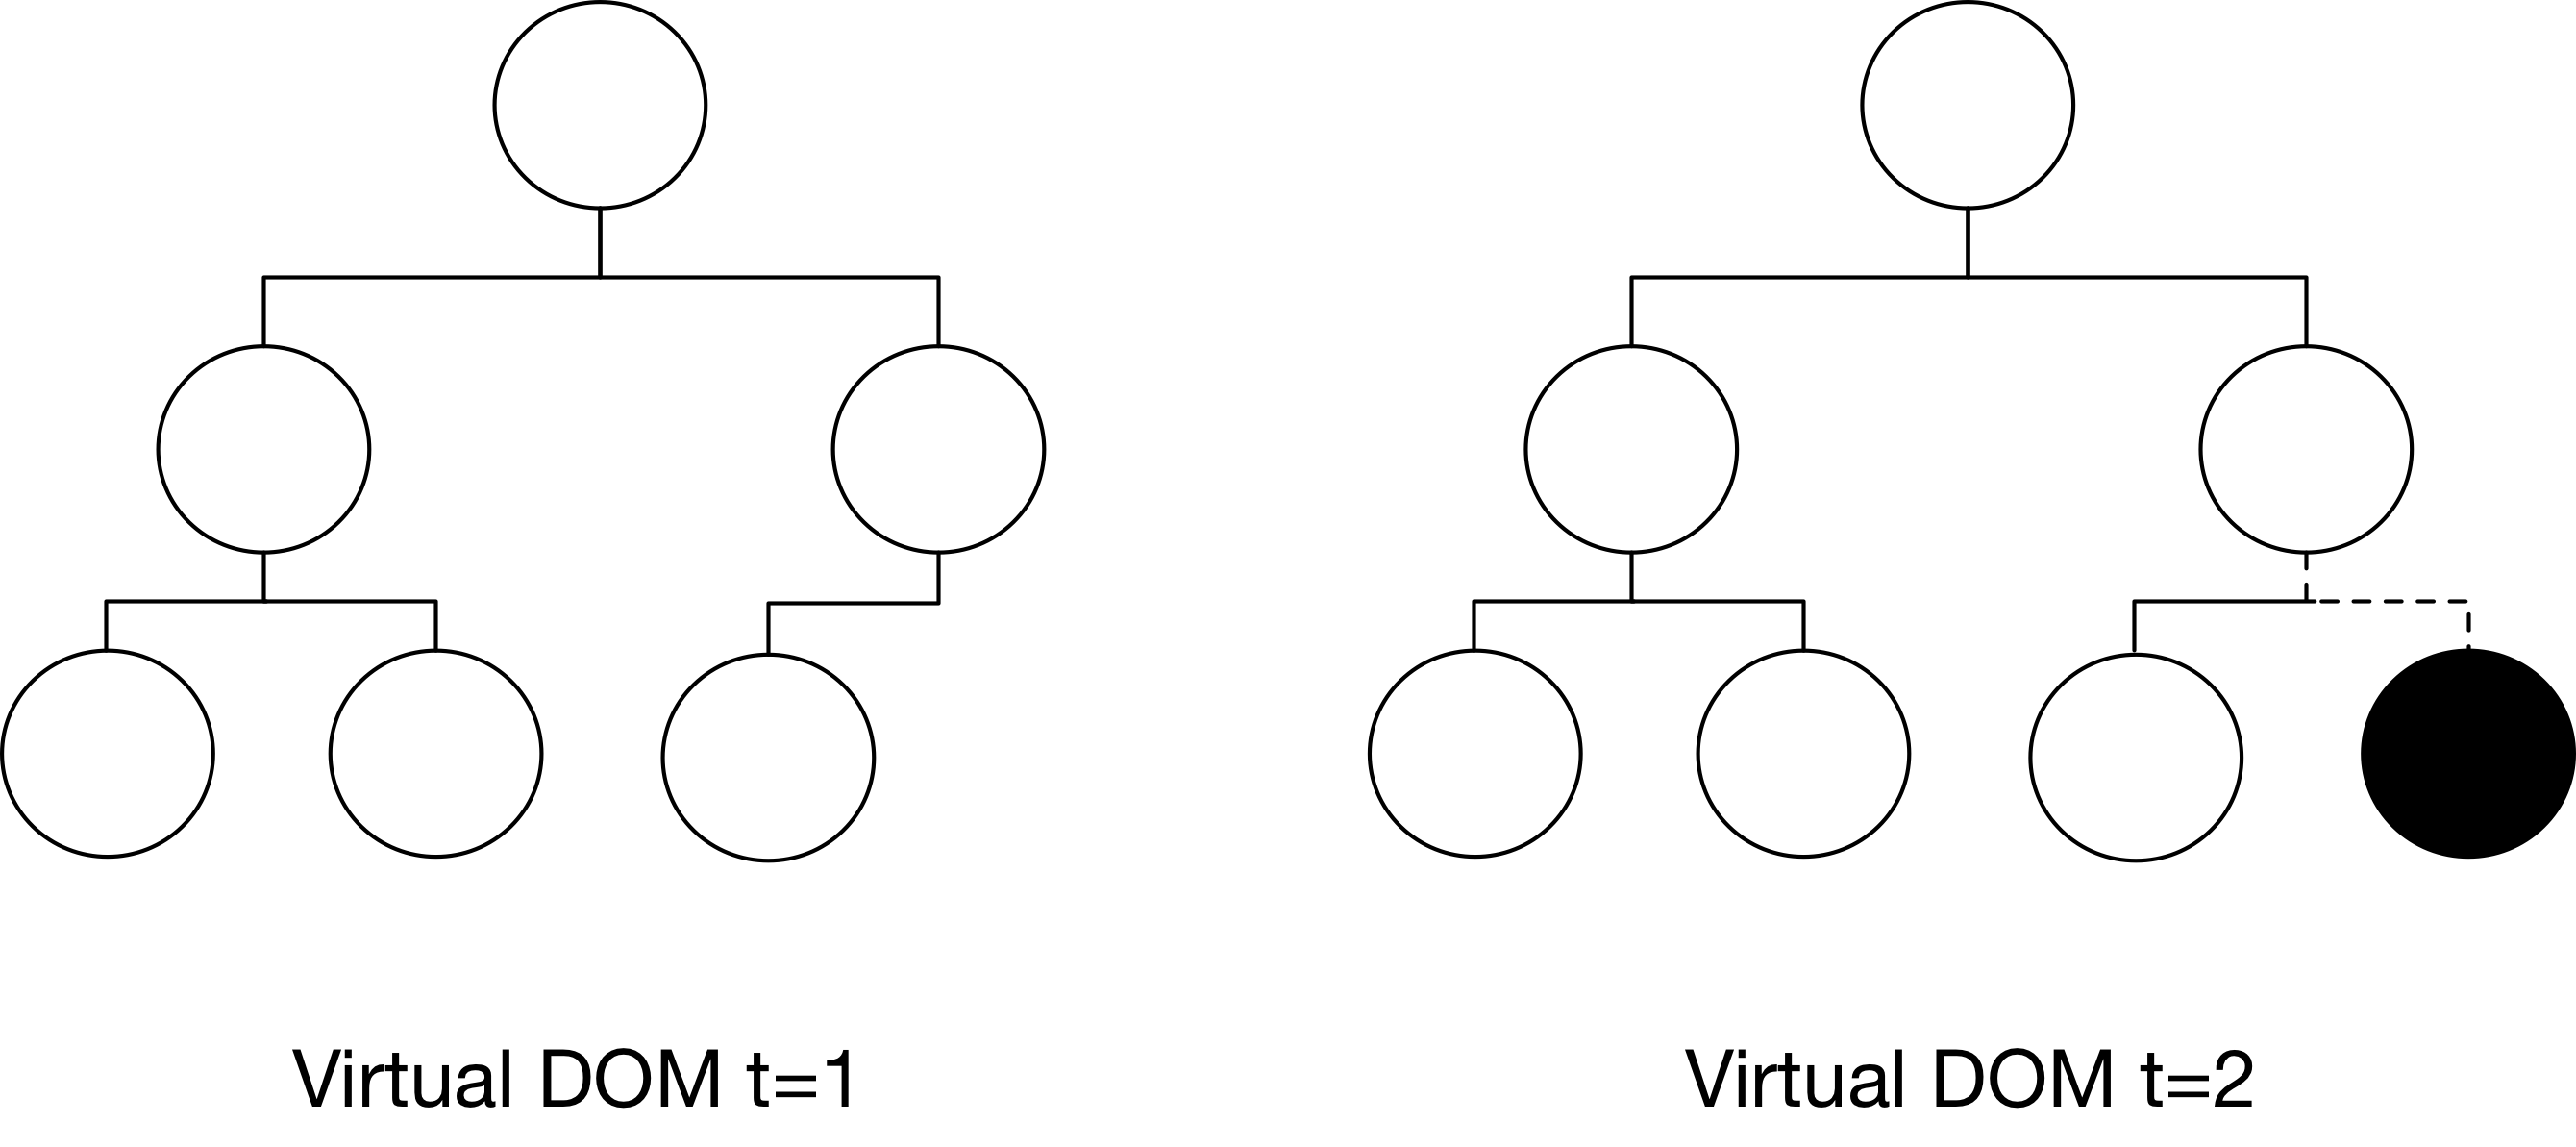
\includegraphics[width=0.8\linewidth]{bilder/grundlagen/VirtualDom.png}
	\caption{Virtual DOM comparison}
	\label{fig:VirtualDom}
\end{figure}

React is a relatively new framework with a new underlaying software architecture for user interfaces. This architecture leads to less files and more encapsulation. Therefore it scales better than classic MVC when having more views on the same data. Due to the Virtual DOM React is really performant when updating the DOM.

\subsection{Redux}

Redux evolves the ideas of the Flux software architecture.
This section is based on the official Redux guide \cite{Redux}.

The primary idea of Redux is to keep all states in a single store.
The only way the state may be changed is by emitting actions.
Actions are objects describing what happened, either at the user interface or at 
the client server interface. So called "pure reducer" functions
define how actions change the state tree.

The major difference between Flux and Redux is that Redux does not have 
a dispatcher and does not support more than one store. With a single root reducer there is just a single store.
In larger applications the root reducer can be split into several reducers,
each operating independently on different parts of the state tree.
 
Redux adds a lot of overhead to an application, more files and code are created. 
Considering that, Redux should only be used if the following points apply.

\begin{itemize}
\item A considerable amount of data is changing over time
\item A single source of truth is needed (all states in one place)
\item Keeping all of the states in a top-level component is no longer sufficient
\end{itemize}

It should further be mentioned that Redux destroys a key principle of React by 
providing access to the state from all components in an application directly. 
It is no longer obvious what data is used in which component (see Fig. \ref{fig:Redux}).
\begin{figure}[H]
	\centering
	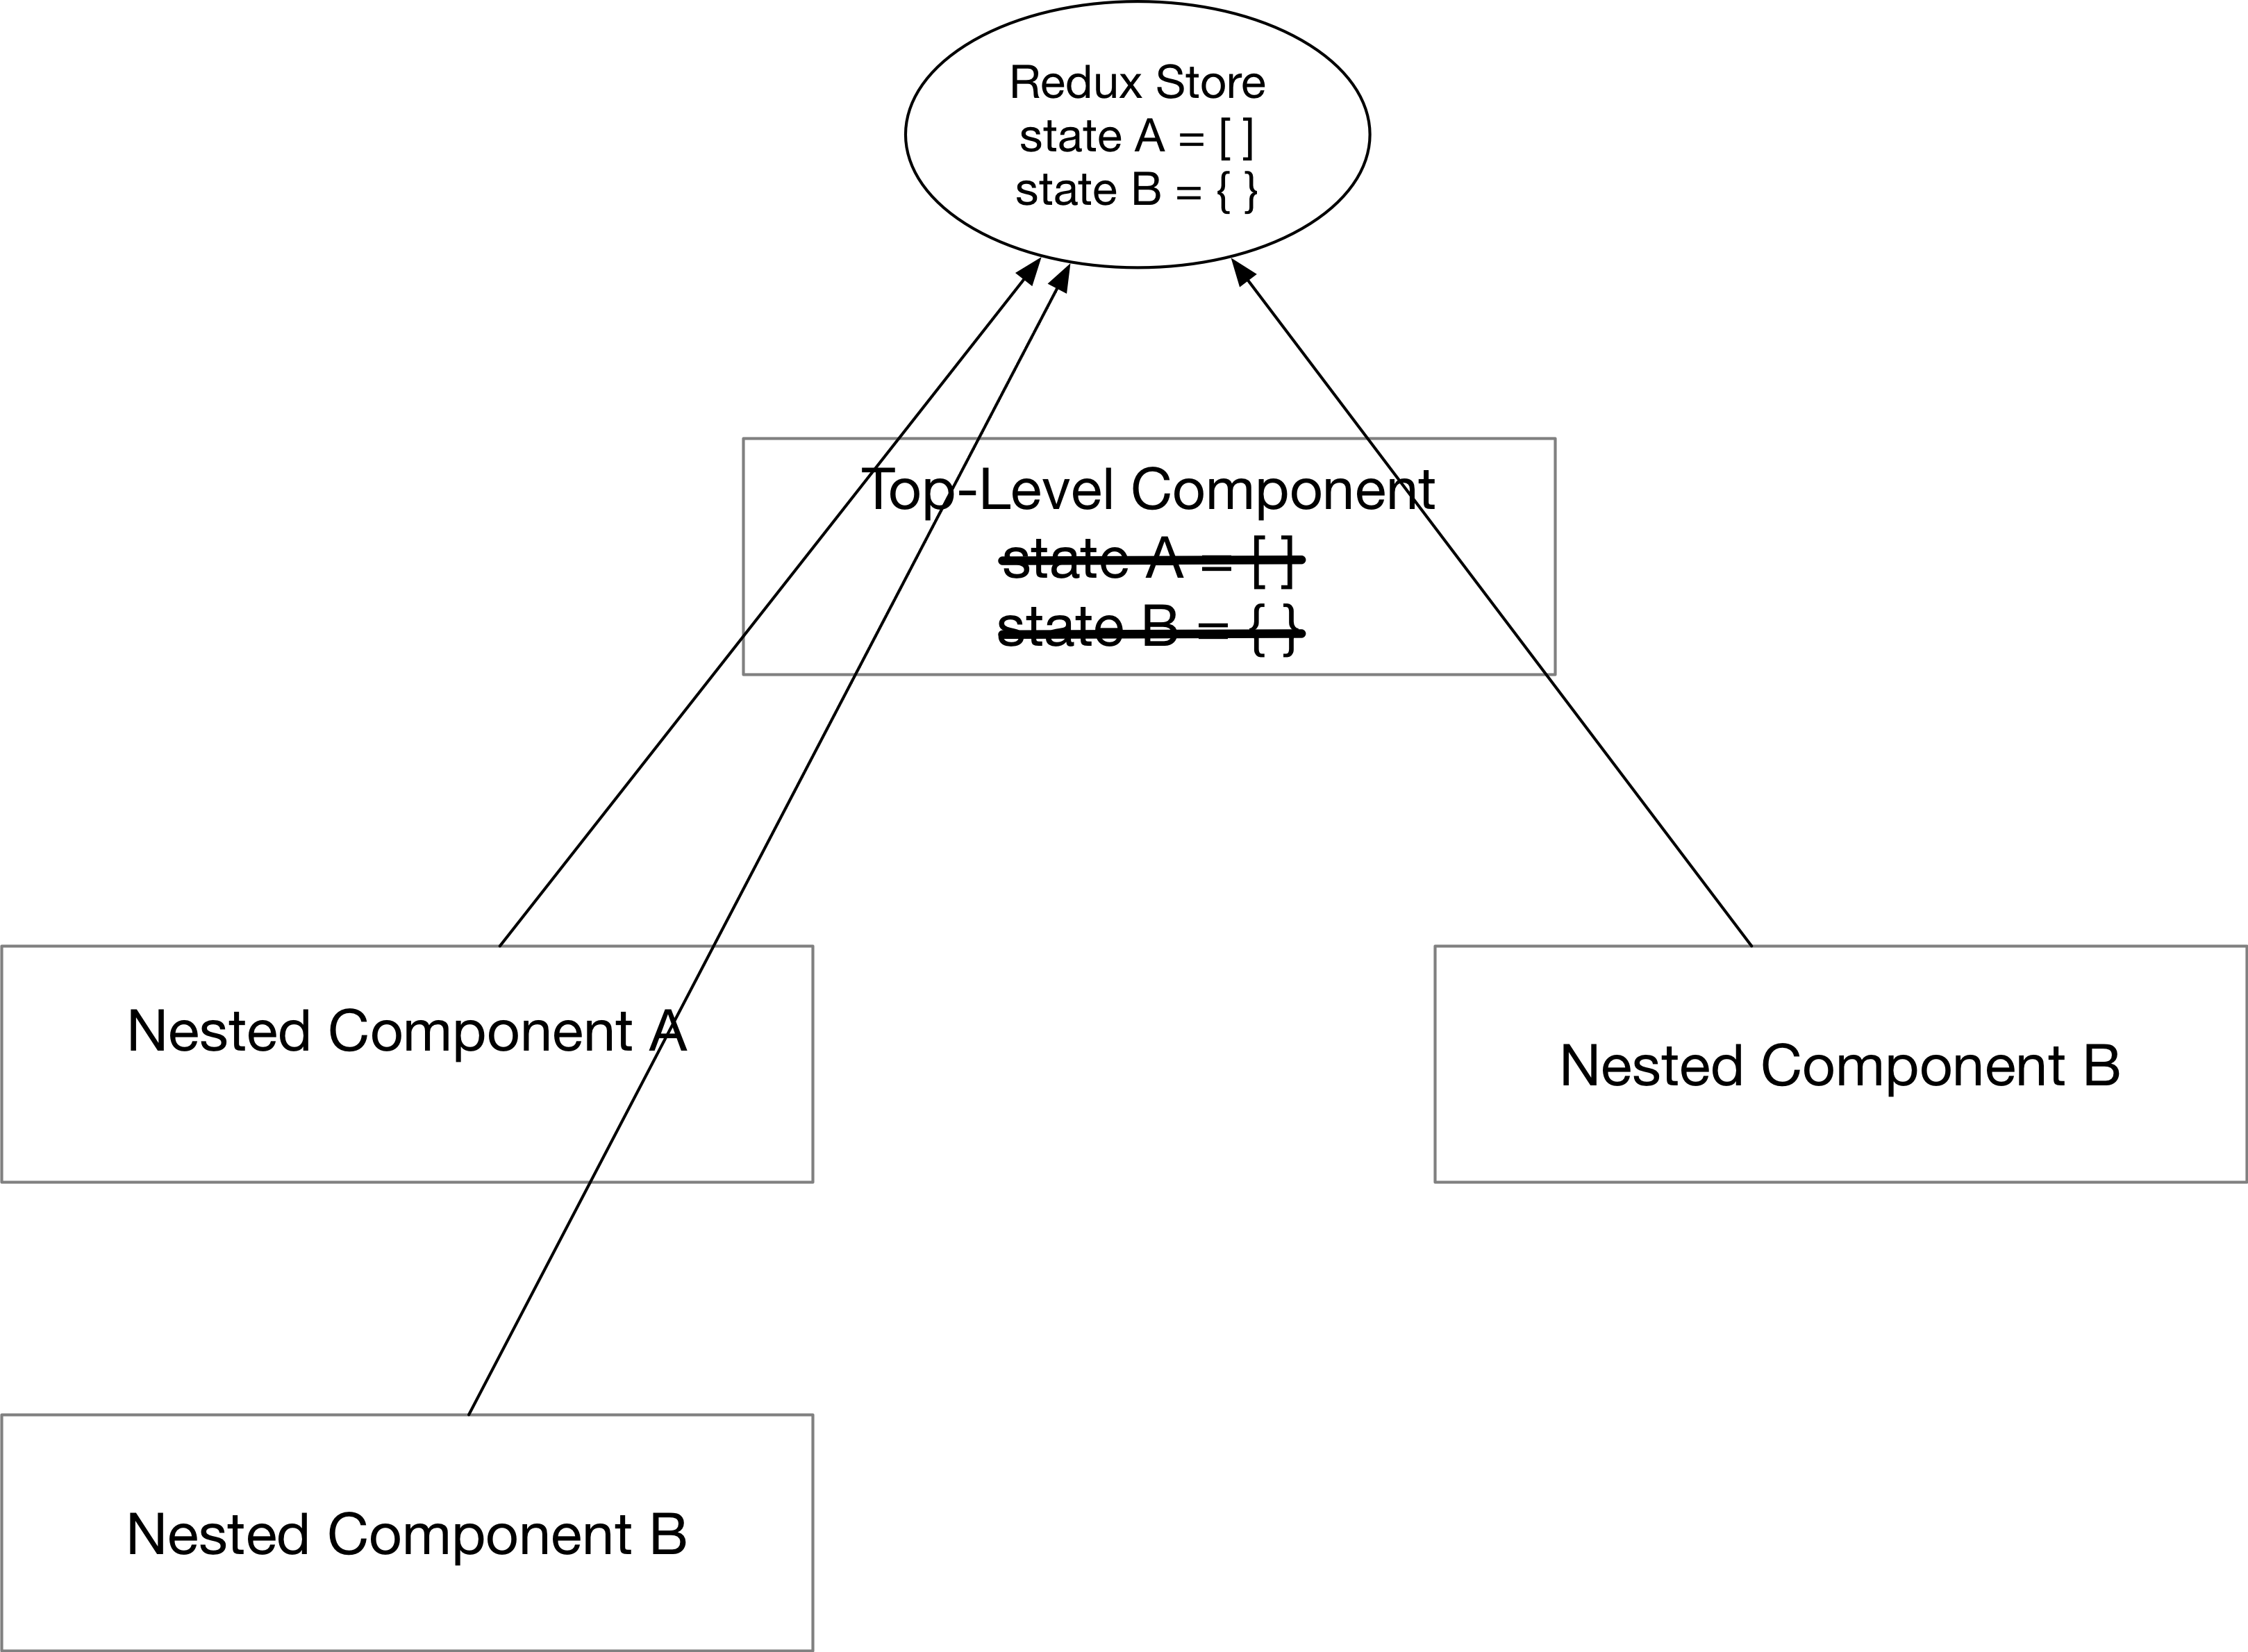
\includegraphics[width=0.8\linewidth]{bilder/grundlagen/reduxStore.png}
	\caption{Redux store}
	\label{fig:Redux}
\end{figure}

\section{TensorFlow.js}
TensforFlow.js is an open source JavaScript library for training and deploying
neural networks in a browser and on Node.js. \index{TensorFlow.js}
First introduced in Spring 2018 it already provides intuitive APIs to build and train models from scratch in a browser.
Existing models can be loaded and re-trained.
Normal TensorFlow models can be imported and used. 

TensorFlow is computation intensive.
It can be significantly accelerated by accessing graphic processors via a WebGl interface.
This facilitates to train a network and execute predictions in a reasonable time. 
In the following we will discuss some core concepts of TensorFlow.js \cite{TenosrFLowJs}. 

\subsection{Core concepts}

Tensors are sets of numbers with an additional shape attribute.
The shape attribute defines the tensors dimensions, 
in other words how to interpret the set as a numerical array.
Tensors are immutable, the values of a tensor can not be changed. \index{tensors}

\lstinputlisting[caption=Tensors]{code/grundlagen/tensor.js}

It is possible to create variables from tensors. Such variables have the same structure as the tensor but they 
are mutable.

\lstinputlisting[caption=Variables]{code/grundlagen/variables.js}

Tensors provide operations that can be performed on them. In TensorFlow.js there is a wide variety
of algorithms that can be applied to tensors.
These operations do not change a tensor, instead they create new tensors.

\lstinputlisting[caption=Operations]{code/grundlagen/operations.js}

TensorFlow.js models are comparable  to functions as they  take inputs and produce outputs.
TensorFLow.js provides a high-level API called \texttt{f.model()} to construct a model with layers.

\lstinputlisting[caption=Model]{code/grundlagen/model.js}

\subsection{Performance}

Even though TensorFlow.js can access the local graphics processing unit (GPU), 
the Tensorflow.js development team reports that TensorFlow implementations 
written in Pyhton or C++ perform 1.5 to 2 times faster.
Small models seem to train faster in the browser, but larger models will 
perform 10-15 faster in Python than on JavaScript \cite{TenosrFLowJs}.

\subsection{Summary}
TensorFLow.js makes constructing neural networks, training and predicting quite easy.
With GPU support such networks run relatively fast even in JavaScript, although 
they are not as performant as TensorFlow distributions
written in C++ or Python. 

TensorFlow.js  distributes the computational load 
across many computers and thereby scales much better than if an algorithm would be running on a single
server, even if that was very performant.

%\chapter{Deep Learning}

Deep learning is a class of neural network optimization methods for networks that have
 a significant number of hidden layers between their input and output layer.
  Compared to learning algorithms of more simple network structures, the methods of 
  deep learning offer a stable learning success even in the presence of numerous hidden layers.

Deep learning has been successfully applied to object detection in computer vision, in natural language processing,
 and speech recognition. In this chapter we will explain how such artificial neural networks 
 function by looking at feed-forward network as an example \cite{Dao}. 

\section{Feed-forward neural networks}

A feed-forward network comprises one input layer, H hidden layers and one output layer.
Each layer consists of a number of elements called "neurons". Each neuron of any given layer is 
fully connected to each neuron
of the previous layer. Mathematically, a neural network is represented by a combination of 
matrix multiplication and
activation functions. An activation function determines when a neuron fires.
It usually is nonlinear. The nonlinear characteristic of the activation function is 
what enables the network to learn. Each neuron in a hidden layer can be described by equations \ref{eq:1} and  \ref{eq:2}

\begin{equation} \label{eq:1}
	y_{j} = f(z_{j})
\end{equation}

\begin{equation} \label{eq:2}
z_{j} = \sum w_{ij}*x_{i} + b_{j}
\end{equation}

\begin{figure}[H]
	\centering
	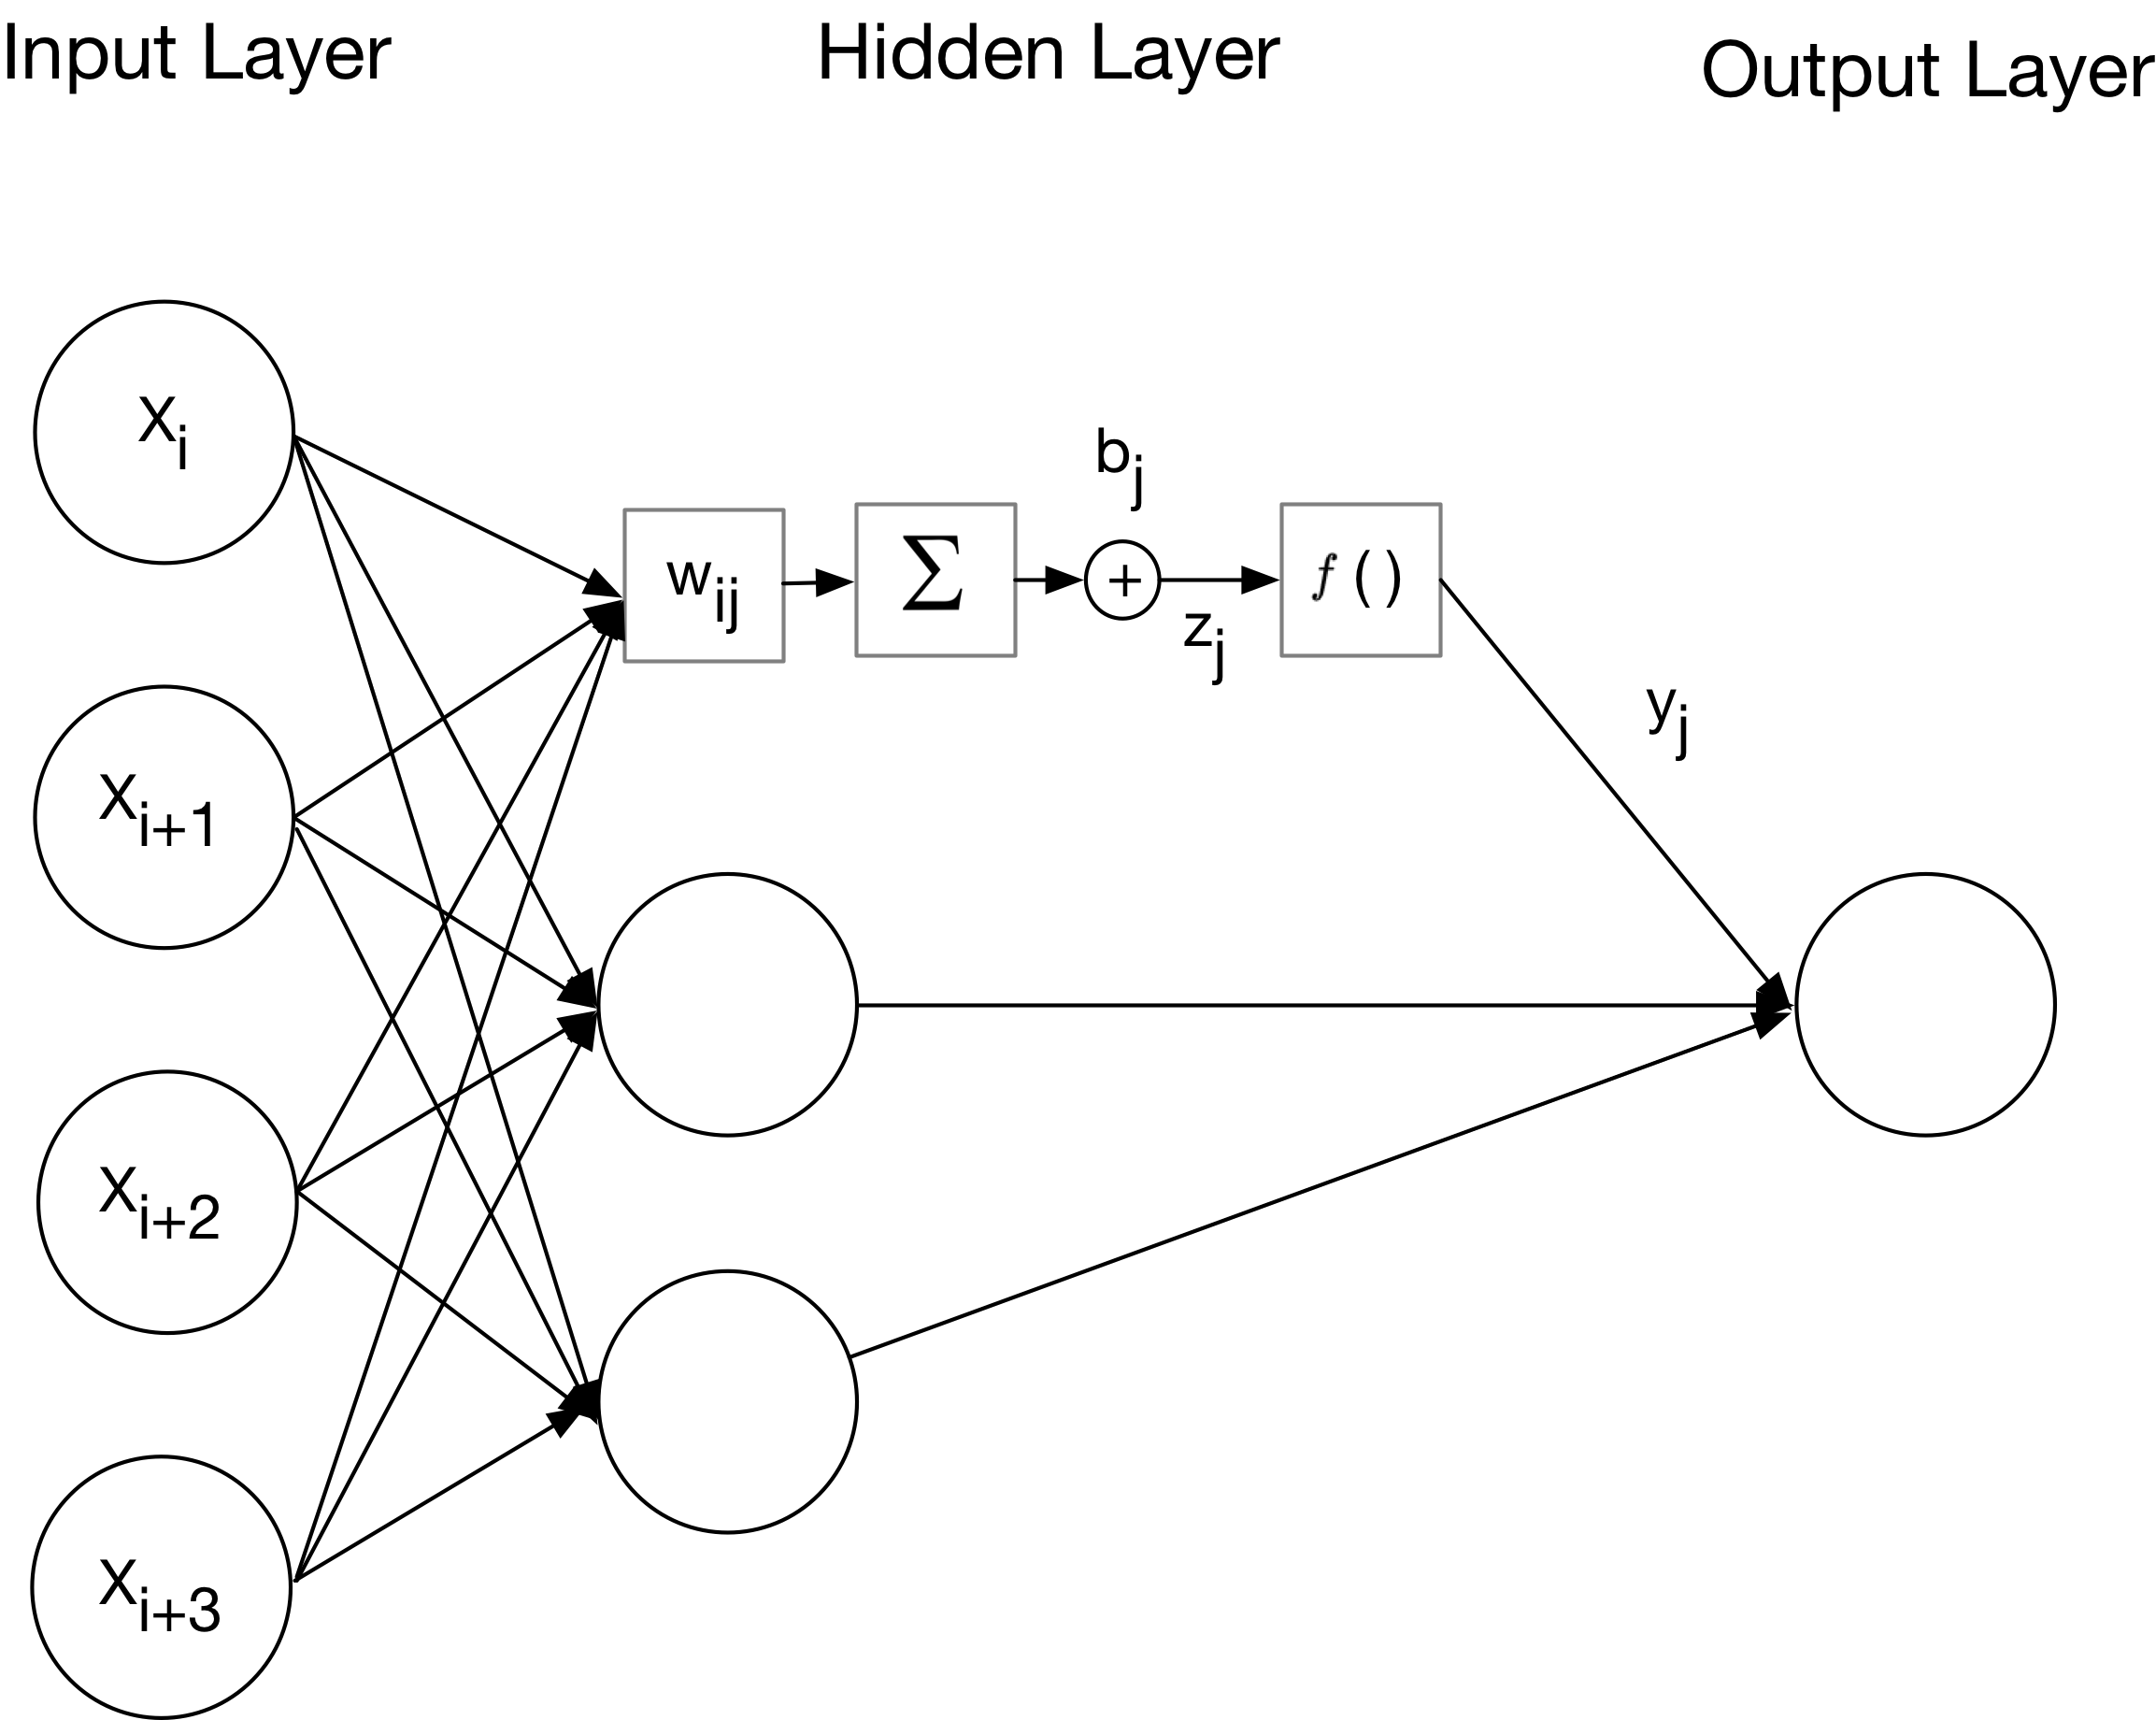
\includegraphics[width=1.0\linewidth]{bilder/grundlagen/fast-forward.png}
	\caption{Schematic view of a  simple two layer fully connected neural network (FCN)}
	\label{fig:FCN}
\end{figure}

The outputs of the preceding layer are each weighted with a weight \(w_{ij}\) before they are accumulated.
The resulting sum is shifted by adding a bias \(b_{j}\) to generate the input \(z_{j}\) for the 
activation function \( f(\cdot) \).
The output of the activation function \(y_{j}\) is then taken as the input for the next 
hidden layer or output layer.
 
 Any continuous functions can be used as activation functions of a neural network. 
 Most common activation functions are sigmoid,  \(f(z) = \dfrac{1}{e^{-z}}\), 
 the hyperbolic tangent, \(f(z) = \frac{exp(z)-exp(-z)}{exp(z)+exp(-z)}\) or the 
 rectifier linear unit (ReLu) \(f(z) = max(0; z)\). ReLu will be used for all future examples.


\begin{figure}[H]
	\centering
	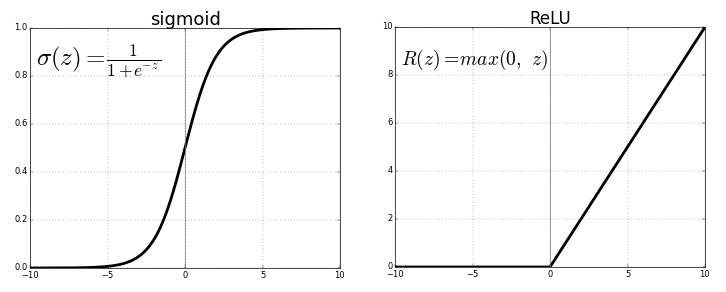
\includegraphics[width=0.8\linewidth]{bilder/grundlagen/sigmoid.png}
	\caption{Sigmoid and ReLu activation function (from\cite{Sigmoid})}
	\label{fig:Sigmoid}
\end{figure}


\subsection{Backpropagation}

Training a neural network means iteratively applying a forward pass followed by an error backpropagation.
During the forward pass the outputs for each neuron are calculated based on its inputs.
The resulting outputs \(y_{out}\) are then compared with the correct answer via a cost function  \(E\).
A common cost function for example is squared error loss (see equation \ref{eq:3}):
 
\begin{equation} \label{eq:3}
	E=\sum\dfrac{1}{2} (target-y_{out}^2) 
\end{equation}

Based on the output of \(E\) it is now possible to check how weights need to be 
adjusted in order to minimize the error.
Applying the chain rule we get equation \ref{eq:4}. 

\begin{equation} \label{eq:4}
	\frac{\partial z}{\partial x} = \frac{\partial z}{\partial y} \frac{\partial y}{\partial x}
\end{equation}

Considering the error  \(E\) we get equation \ref{eq:5}

\begin{equation}  \label{eq:5}
\Delta_{W}E =
\frac{\partial E}{\partial W_{l}} =
\frac{\partial E}{\partial y_{out}}
\frac{\partial y_{out}}{\partial z_{out}}
\frac{\partial z_{out}}{\partial y_{n-1}}
\frac{\partial y_{n-1}}{\partial z_{n-1}}
\end{equation}

Using the calculated gradient $\Delta_{W}E(y_{out})$  it is now possible 
to determine the next weight matrix update using a gradient descent (equation \ref{eq: 6}):

\begin{equation} \label{eq:6}
W_{l}^{t+1}=
W_{l}^{t}-\eta\Delta_{W_{l}^{t}}E(y_{yout)}
\end{equation}

where \(W^{t}\), \(W^{t+1}\) are the current and the updated weight matrices, respectively,
and  \(\eta\) is the learning rate.

\subsection{Weight update}
Calculating the gradient for a complete dataset can take a lot of computation time.
To reduce the amount of computation required
mini-batches can be used to calculate the gradient only based on a few sampled data points. 
Using this analytic gradient a parameter update is performed. There are several ways to perform this update,
the most common one being the stochastic gradient descent (SGD).
In this algorithm, parameters are simply changed along the negative gradient 
direction in order to minimize the error.


\subsection{Initialization}
A neural network needs its weights initialized before it can be trained.
Random initialization is the most common way to create the initial weights.

\subsection{Batch normalization}
To avoid numerical problems due to extreme values the input data is 
normalized (see equation \ref{eq:7}).

\begin{equation}\label{eq:7}
	x \Rightarrow \hat{x} = \dfrac{x-\mu}{\sigma} \Rightarrow x_{norm} = \gamma \hat{x} + \beta
\end{equation}

\(\mu\) and \(\sigma\) are the mean and the  standard deviation of the dataset, respectively. 
\(\gamma\)\ and \(\sigma\) scale and shift the parameters. Batch normalization accelerates 
training time and makes a deep neural network less sensitive to initialization issues.

\section{Classification}
A common task for neural networks is the classification of images, or more general the classification of data into a specific category. The best performing neural network architectures for classifying images are 
convolutional neural networks (CNN). 
All convolutional neural networks consist of convolutional layers followed by pooling 
layers and some fully connected layers.

\subsection{Convolutional layer}
In a convolutional layer several kernels are applied to extract spacial related features. Each output from the the convolutional layer is called a feature-map. Each feature-map was created by a different convolutional kernel of the layer. 

\begin{figure}[H]
	\centering
	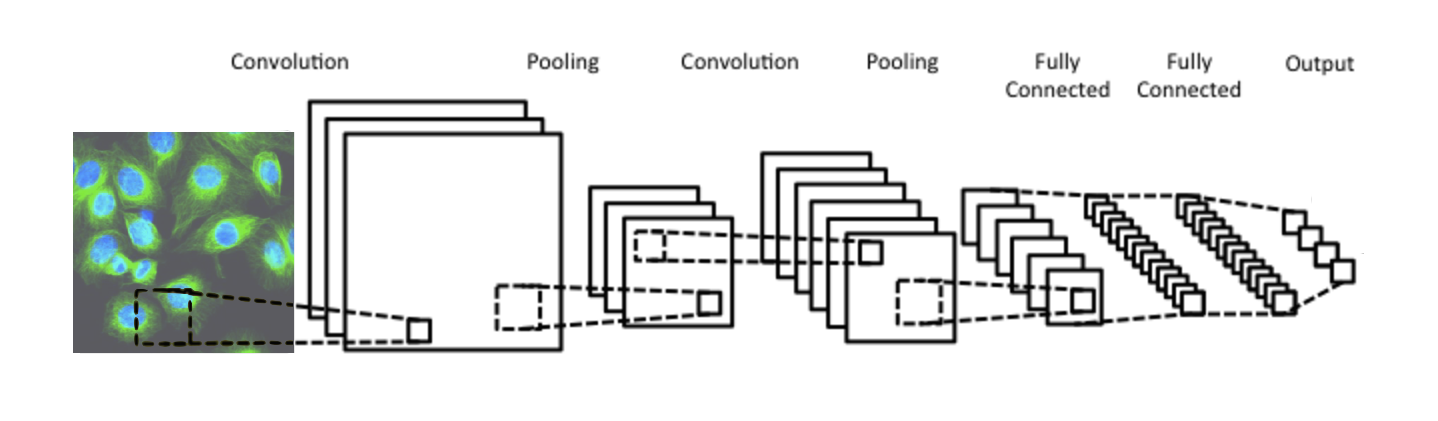
\includegraphics[width=\linewidth]{bilder/grundlagen/convolution.png}
	\caption{Schematic view of a Convolutional Neural Network (CNN) (from \cite{Dao})}
	\label{fig:CNN}
\end{figure}

\subsection{Pooling layer}
After features have been extracted into feature maps,  the pooling layer reduces the 
size of the feature maps and makes them computationally  tractable. A simple implementation 
of a pooling layer is the max-pooling layer, which uses a sliding windows over the input and 
selects the maximum of each window.

\begin{figure}[H]
	\centering
	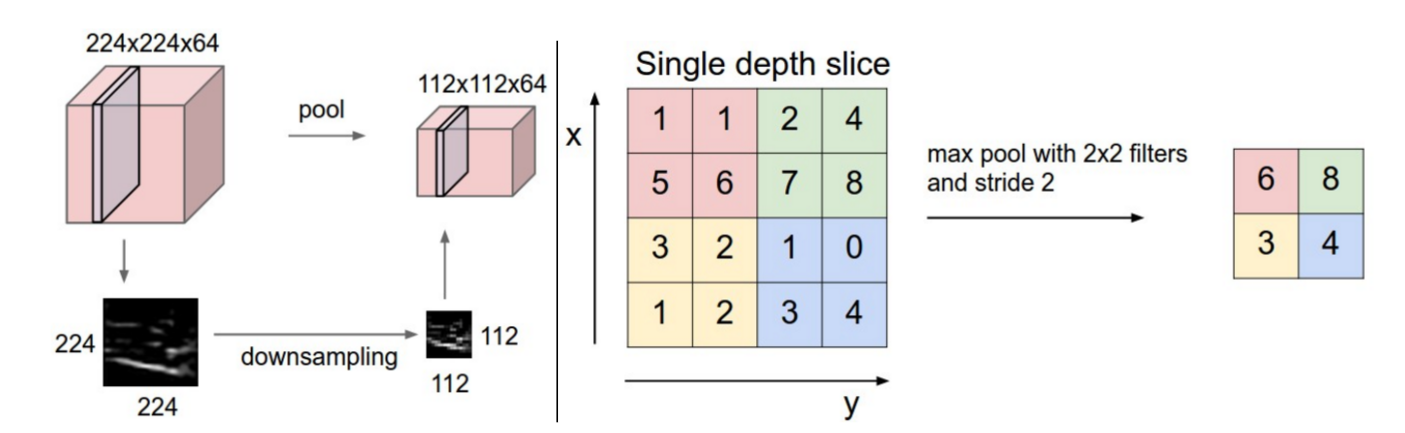
\includegraphics[width=\linewidth]{bilder/grundlagen/pooling.png}
	\caption{Pooling layer (from\cite{Dao})}
	\label{fig:Pooling}
\end{figure}

\subsection{Data augmentation}
Convolutional neural networks need a lot of data to generate satisfactory output. \index{data augmentation}
If not enough data can be provided the data can be artificially augmented by using different approaches.
images can be turned or flipped, cropped, blurred or even resized. This makes it 
possible to generate a lot of data which can be used to further improve training.

\begin{figure}[H]
	\centering
	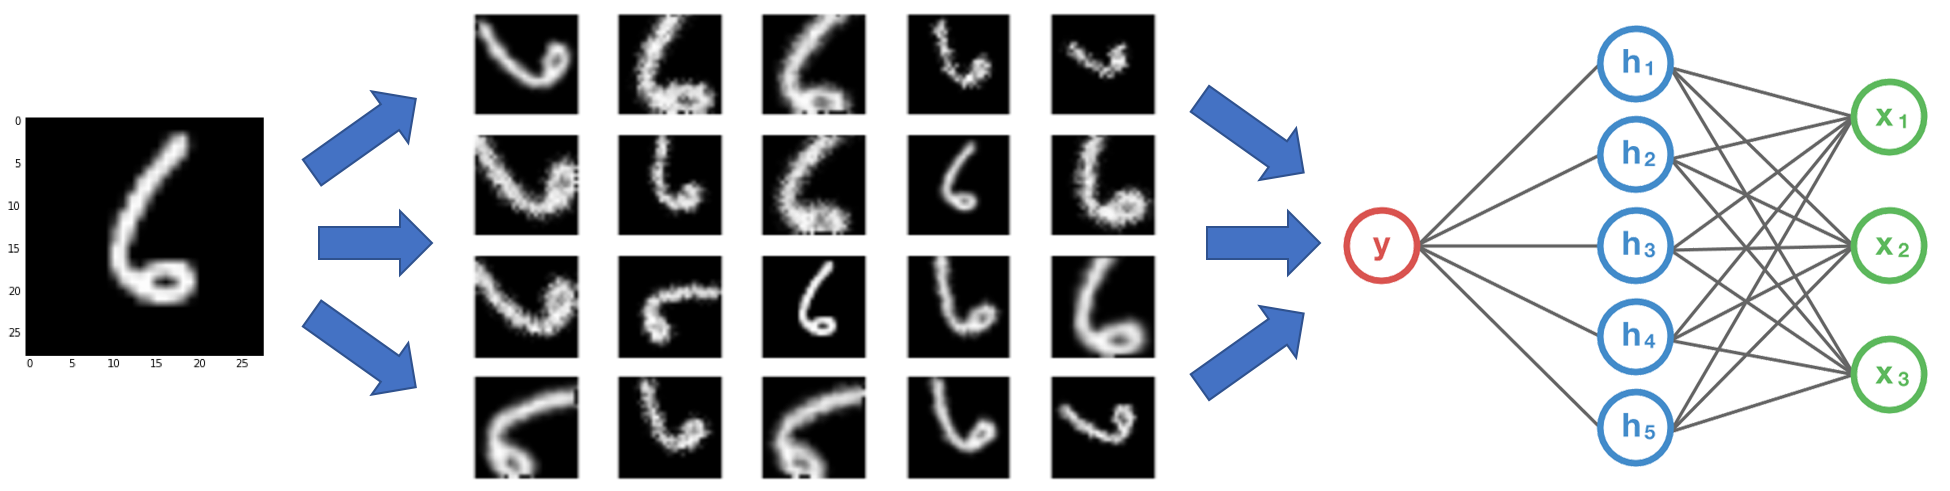
\includegraphics[width=\linewidth]{bilder/deep_learning/data_aug_basic.png}
	\caption{Data augmentation(from  \cite{Ratner2017})}
	\label{fig:COMPONENT}
\end{figure}


%\chapter{Image Based Profiling}

Modern fluorescence microscopy combined with high throughput biotechnology, automatically quantifying biological properties in images, is now widespread. They provides new insights into human cells and are powerful technologies for studying cell biology. 
Using this technology more than more than 
one hundred thousand  images can be produced per day.
This makes automated image analysis a necessity. 
Image-based profiling aims at getting as much data 
as possible from a biological sample and to encoding
it in a proper way. Image-based profiling experiments capture a wide range of data
from biological samples without prior knowledge
of the existence of any markers.
Data mining and machine learning techniques can then be applied to identify patterns \cite{Jones} \cite{Scheeder2018}.

\subsection{Drug discovery}

One important application of image-based profiling is identifying biological mechanisms of actions (MOA),
for example checking damage of DNA replications due to chemical perturbations.
When developing new drugs and making predictions about unknown
chemical compounds it is important to know what chemical compounds cause which biological mechanisms of action.
Morphological profiles can predict these MOAs for chemical compounds.

\subsection{Typical workflow}

There are two approaches in image-based phenotyping of perturbations. 
It should be considered that they are different.
The first approach is called phenotypic screening. 
Phenotypic screening uses pre-defined, specific phenotypes which are compared 
with the specimen in order to identify drugs or drug targets that might have affected 
them.

The second method is called profiling of perturbations. 
Here a computer is trained with a large set of samples, both
affected by perturbations and unaffected ones.
Once trained the computer can analyze new specimen 
and for perturbed ones identify the drugs or drug targets that have affected them.
This approach doesn't require the specification of any features such as cell size, intensity, shape, or texture.
It furthermore permits how any specimen would look if it was affected by a specific perturbation.


\begin{figure}[H]
	\centering
	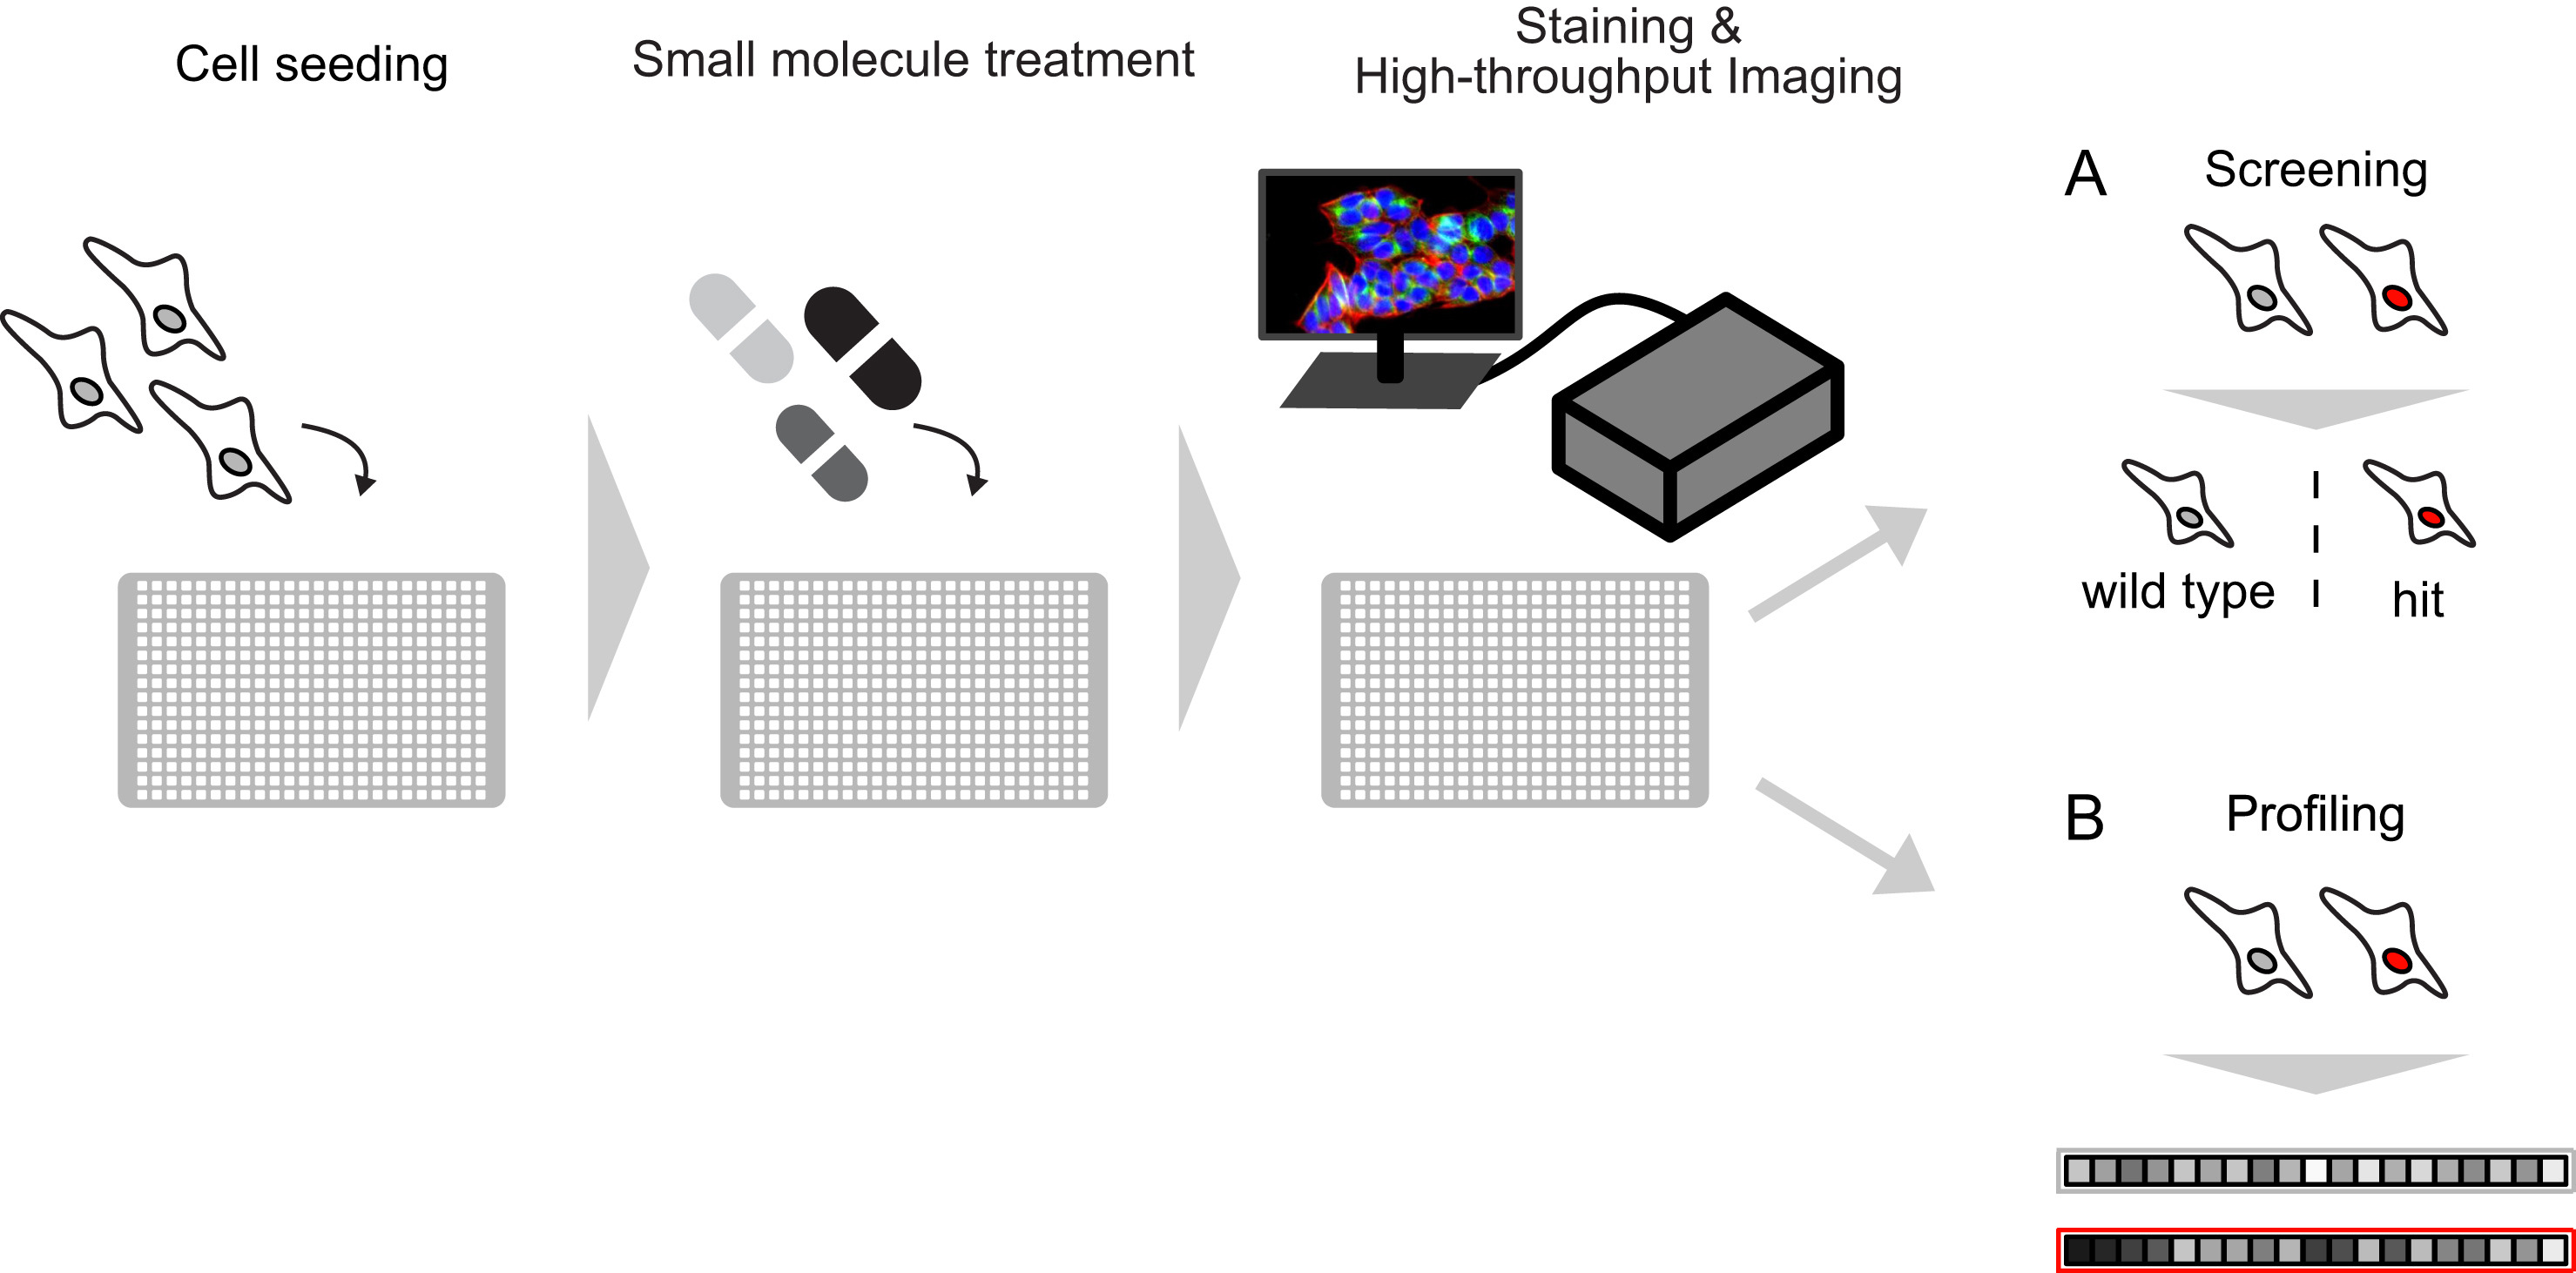
\includegraphics[width=0.8\linewidth]{bilder/cells/hcu.png}
	\caption{Typical workflow of image-based small molecule experiments (from \cite{Scheeder2018})}
	\label{fig:Workflow}
\end{figure}

Fig. \ref{fig:Workflow} illustrates a typical workflow of image-based small molecule experiments. First cells need to be attached to plates. In a second step cells are perturbed. Then after staining the cells, images are taken using automated microscopes. At the end either screening approaches (A) or (B) profiling approaches can be used to classify perturbed cells.

\subsubsection{Segmentation}

Small molecule profiling is based on staining subcellular structures (Fig. \ref{fig:ig:Segmentation}).
An accurate segmentation of cells can be achieved by in intensity-based thresholding and other approaches. A number of computational applications for segmentation-free analysis in image-based profiling have been developed, the most famous one being the Cell Profiler \cite{CellProfiler}.


\begin{figure}[H]
	\centering
	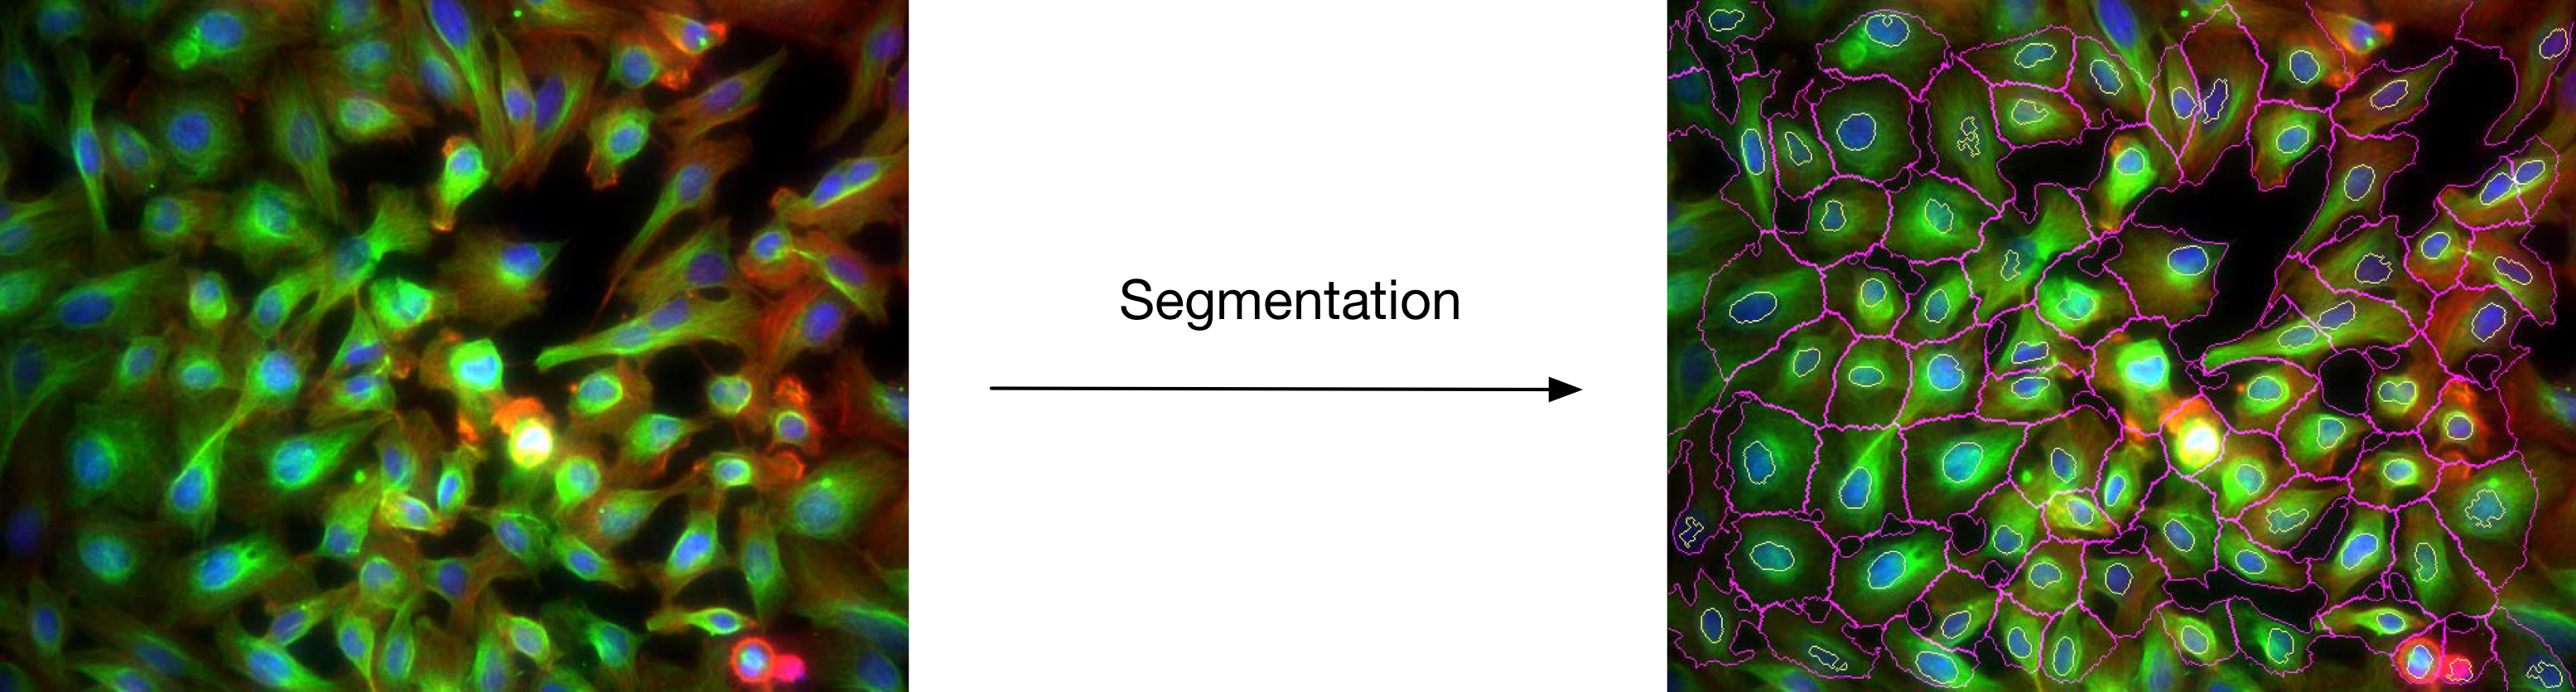
\includegraphics[width=0.8\linewidth]{bilder/cells/segmentation.png}
	\caption{Segmentation (from \cite{Pau})}
	\label{fig:Segmentation}
\end{figure}


\subsubsection{Classification}


A typical objective for profiling experiments is the classification of compounds that cells have been perturbed with. 
Common classifiers are random forests and deep neural networks that are employed to achieve higher 
accuracy in predicting biological MOAs.


\begin{figure}[H]
	\centering
	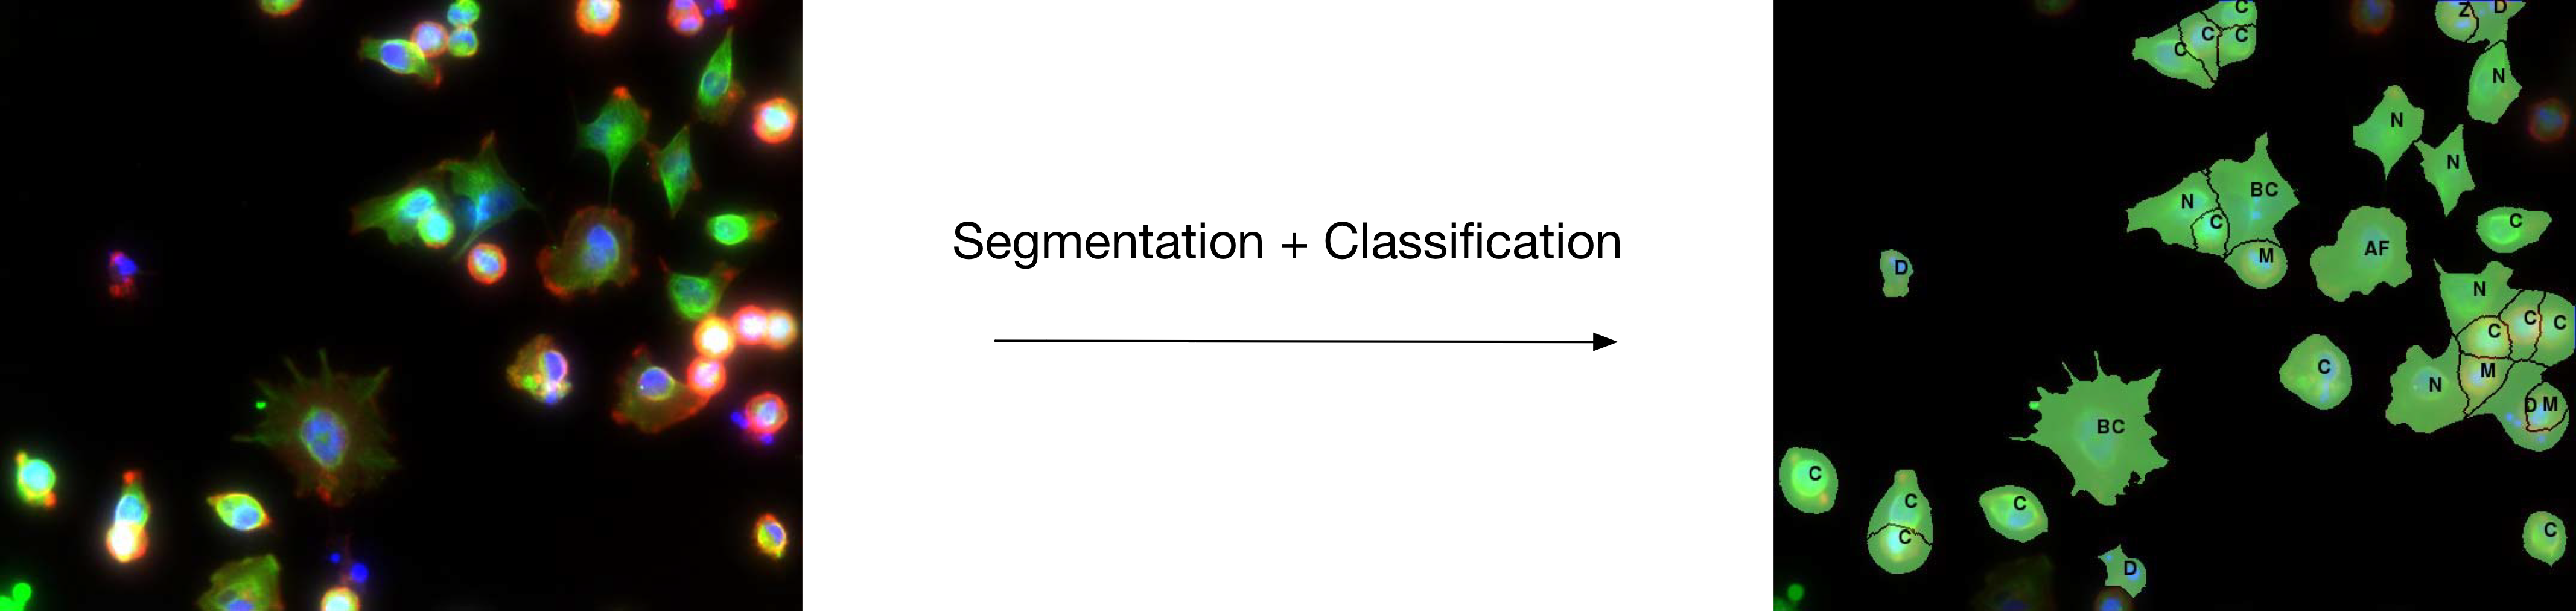
\includegraphics[width=0.8\linewidth]{bilder/cells/classification.png}
	\caption{Classification  (from \cite{Pau})}
	\label{fig:Classification}
\end{figure}





%\chapter{Related work}
This chapter is about presenting CellProfiler Analyst (CPA), a first generation tool for interactive 
data exploration and classification of large biological image sets. 
It was first introduced in 2016 at the Broad Institute of MIT and Harvard. 
The following section gives an overview of CPA's main functionality and an exploration of its key features, 
the classifier and image gallery. 

This project is highly influenced by CPA and basically aims to improve it and make it accessible
to anybody without having to install any software. CPA is free and open source, 
available at \href{http://www.cellprofiler.org}{http://www.cellprofiler.org} and from GitHub under a 
BSD-3 license. It is available as a packaged application for
Mac OS X and Microsoft Windows and can be compiled for Linux.

\subsection{CellProfiler Analyst}
CPA is a GUI based tool. It provides features for data exploration and classification via 
its user interface. There are only a few comparable tools for this purpose, the most prominent being  
Ilastik, CellCognition and WND-CHARM.

All these tools lack a suitable companion visualization tool capable of handling large datasets. 
Furthermore they do not provide selectable classifier algorithms. Another big benefit CPA has compared 
to all other existing tools that it incorporates an interactive object classification and image viewing feature.

\begin{figure}[H]
	\centering
	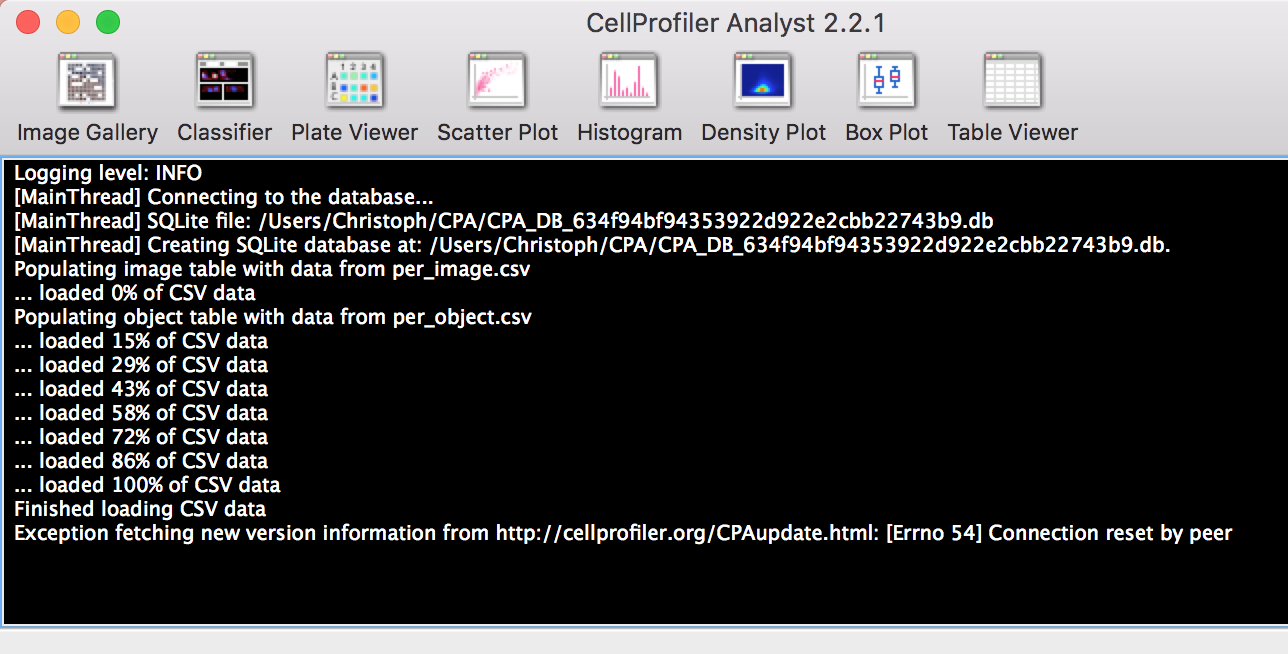
\includegraphics[width=1.0\linewidth]{bilder/related_work/cpa_main_view.png}
	\caption{CPA main view, different views are selectable  (from \cite{Jones2008})}
	\label{fig:CPA}
\end{figure}

\subsection{Classifier}
The Cell Profiler Analyst Classifier makes it possible to create categories and to classify cells.
 After fetching images from a predefined dataset it is possible to classify images 
 by simply drag and dropping them on a category. Multi-select features are also implemented
  and enable to drag and drop multiple images at the same time. 
  
  Further it is possible to add an unlimited amount of categories by clicking the "add category" button. 
  After annotation is done the algorithms can be trained. Once training is done more images can be 
  fetched and then be automatically annotated by clicking the "evaluate" button. 
  
  If results do not suffice further images can be annotated to train the algorithm. 
  Different algorithms can be used to classify the uncategorized images, such as 
  RandomForest Classifier and AdaBoost Classifier.

\begin{figure}[H]
	\centering
	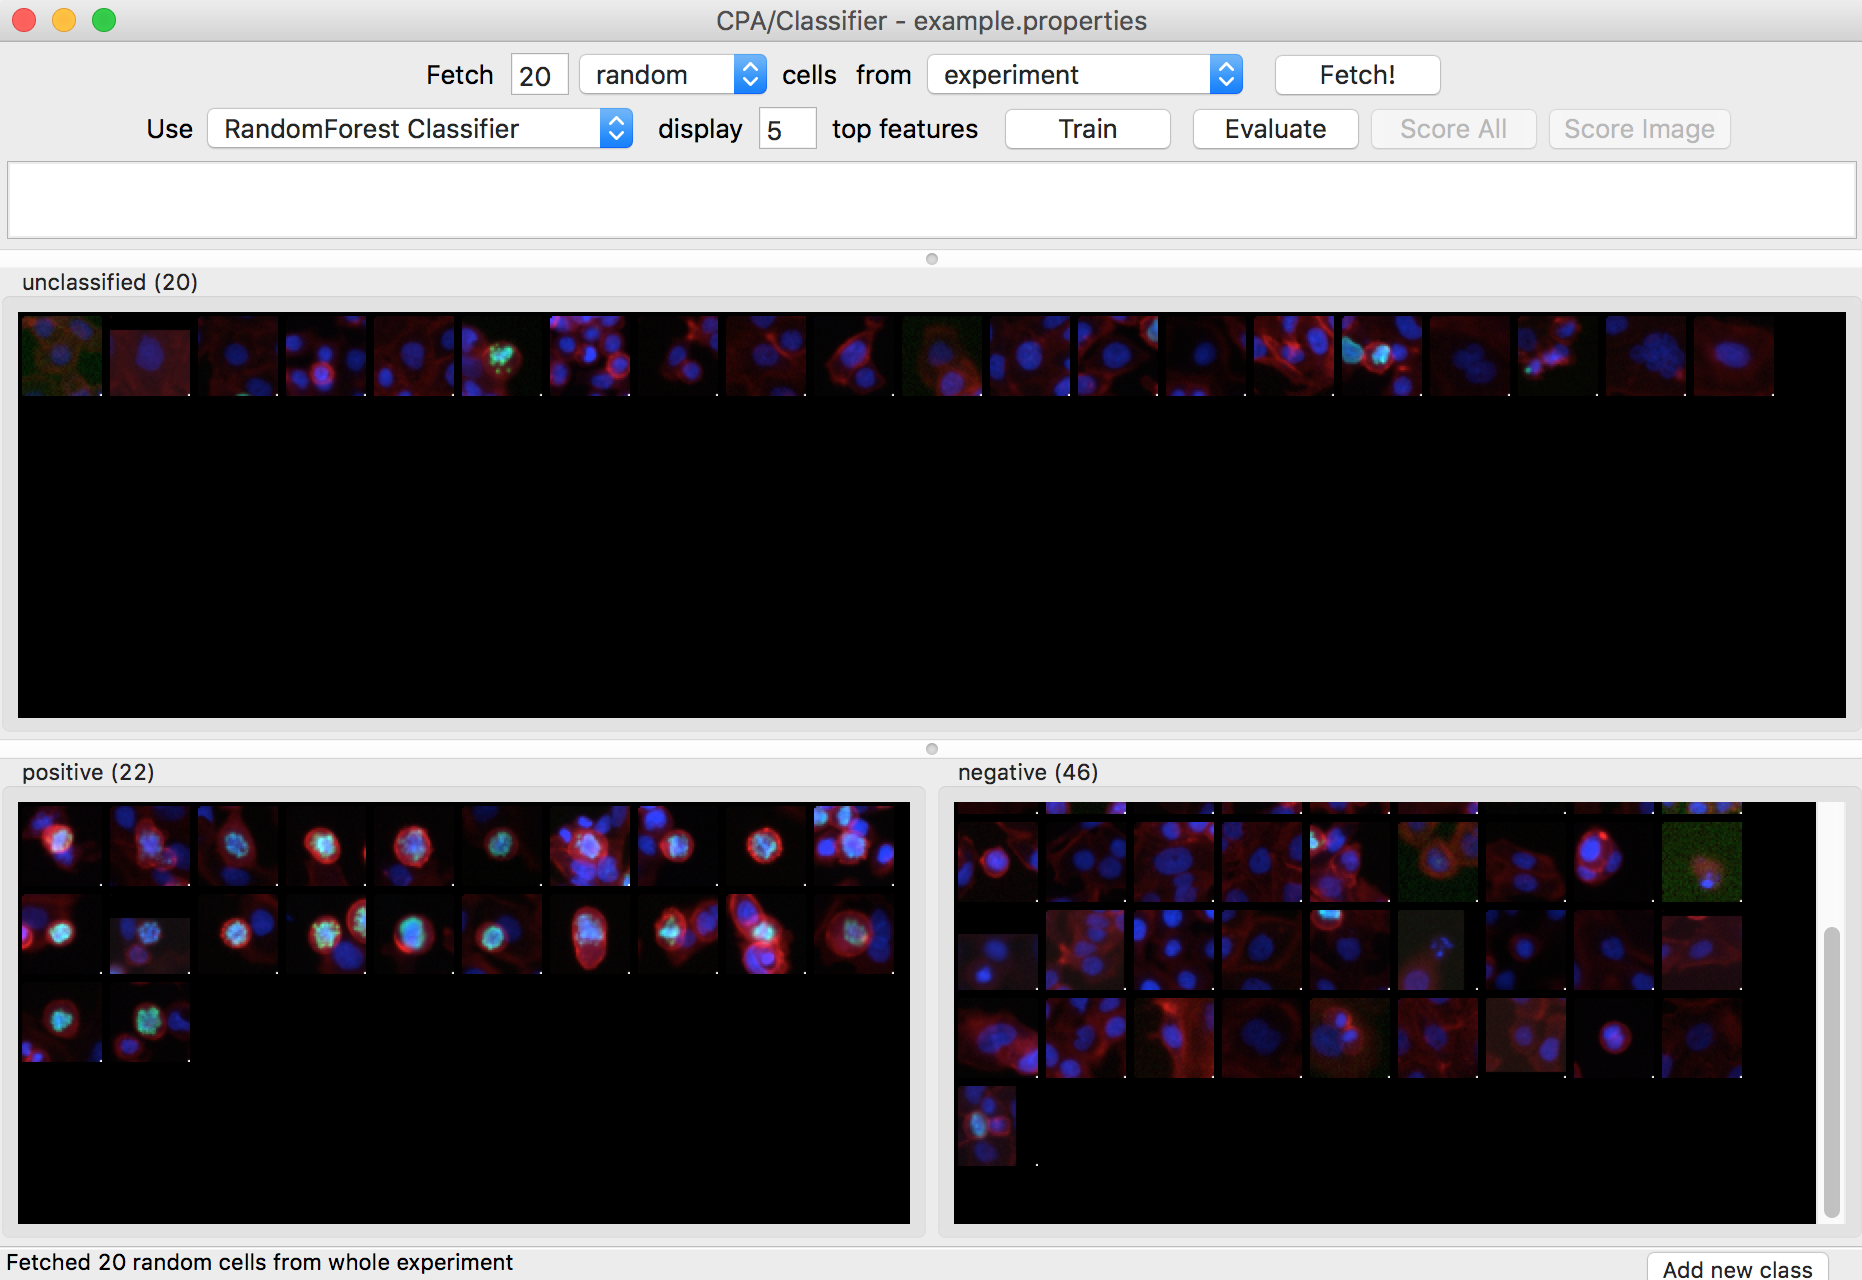
\includegraphics[width=1.0\linewidth]{bilder/related_work/classifier.png}
	\caption{CPA classifier view (from \cite{Jones2008})}
	\label{fig:Classifier}
\end{figure}


\subsection{Visualization}


In order to explore a dataset and to predict and validate a result, a good visualization is needed. 
CPA offers different ways of displaying data and results. 

One simple visualization possibility is the Image Gallery where images from the dataset can be selected and 
displayed in their original size. Filters can be applied to only select images with experiment specific meta data. 
There are many more ways to display and explore data in CPA.

\begin{figure}[H]
	\centering
	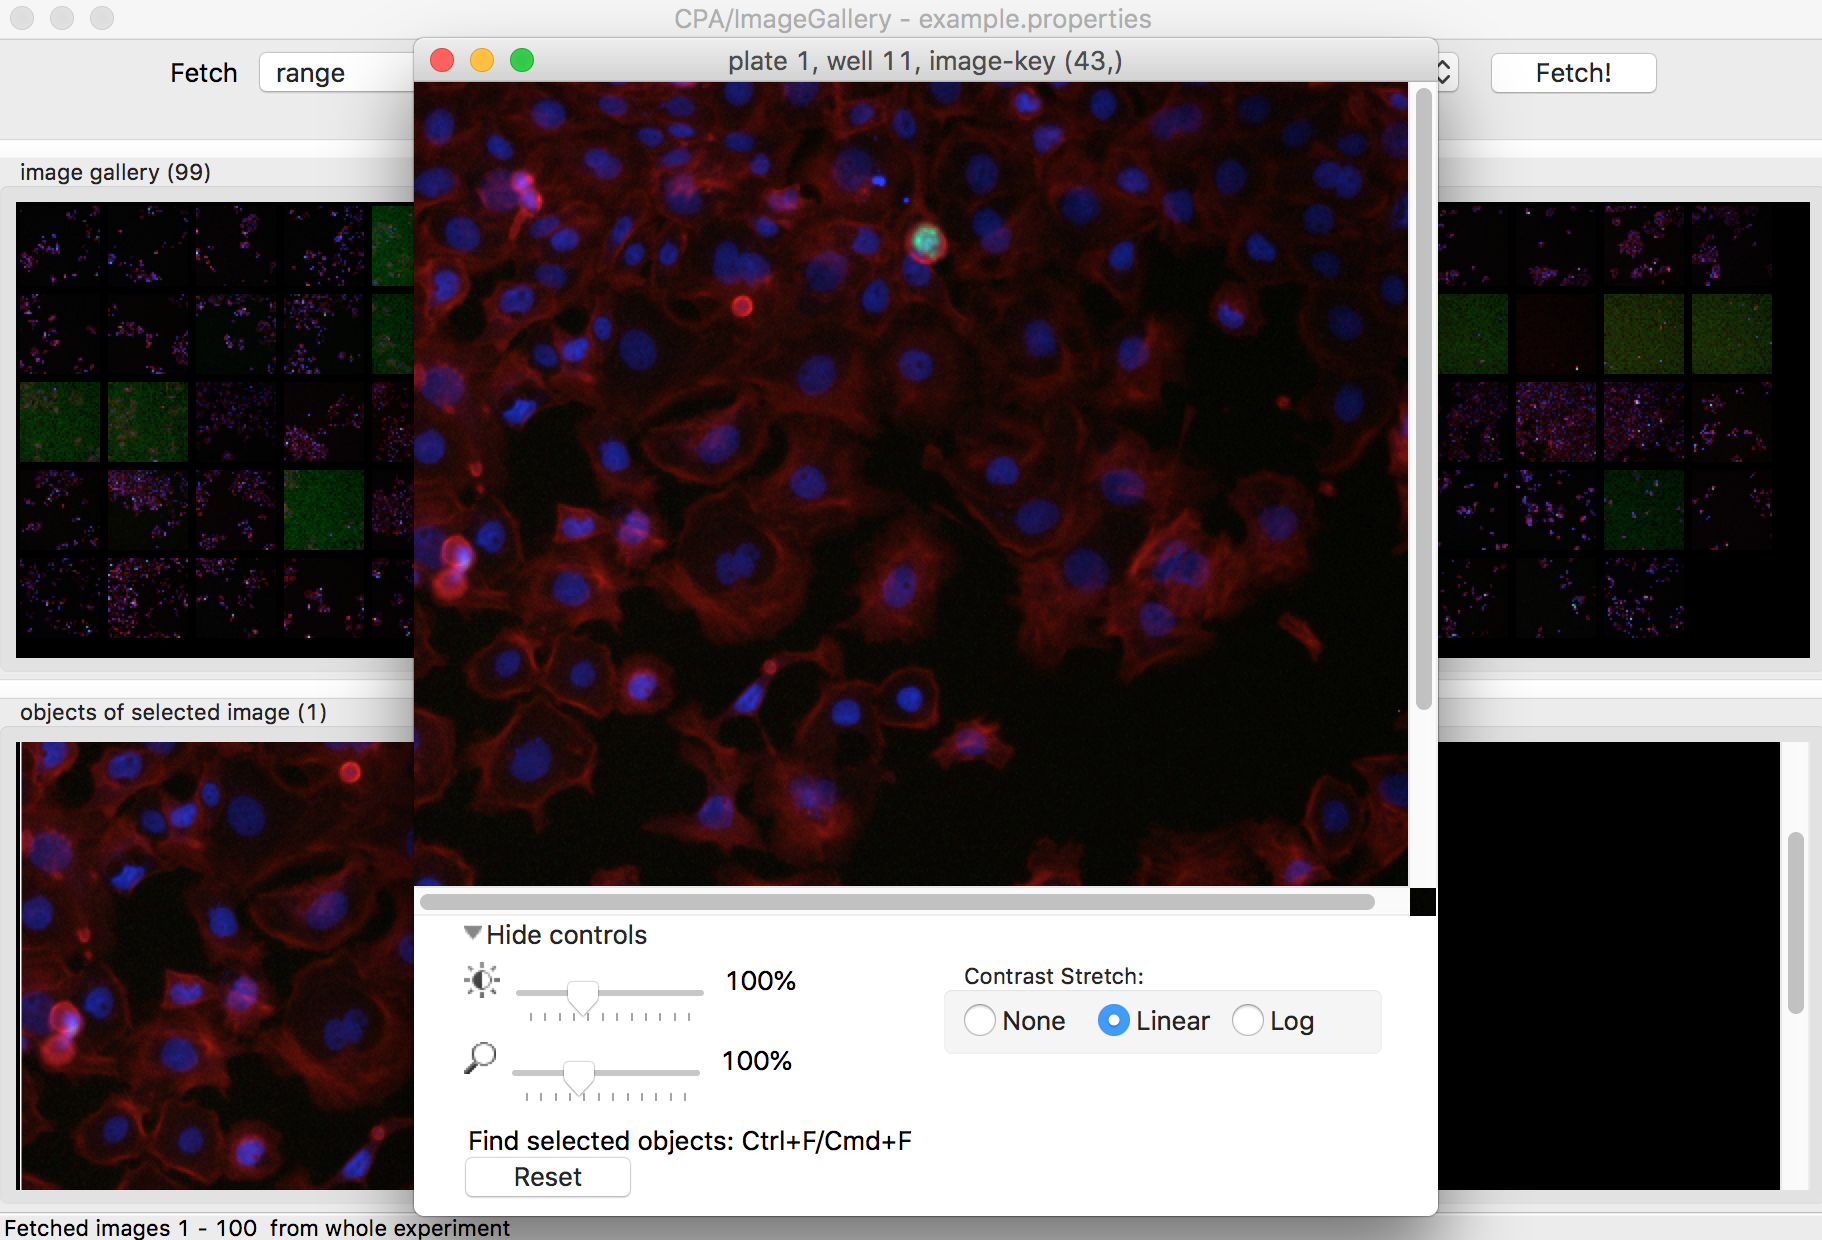
\includegraphics[width=1.0\linewidth]{bilder/related_work/visualization.png}
	\caption{CPA Main View Different Views Are Selectable (from \cite{Jones2008})}
	\label{fig:RL}
\end{figure}


\subsection{Downsides of CPA}
Getting CPA to run on a computer requires installation first. This installation is
not trivial as the system requires a MySQL database system to work.

Furthermore, the powerful user interface makes the system complex and difficult to use. This can 
scare off potential users.






%\chapter{CYTO AI}
CYTO AI is the first fully web-based image labeling and classifying tool there is. 

With React and TensorFlow.js a fully web-based design was possible. No installation of databases or any configuration is needed to use all advantages of modern machine learning and labeling.
No data will be uploaded to any server, all data never leaves the browser which makes CYTO AI very performant and sets a high standard of privacy at the same time.
The following sections shall explain how CYTO AI works and which techniques and architectures were used to build it.

\subsection{System overview}
First pictures need to be uploaded by clicking on the upload button, whole folders can be selected. Mind that also all images in subfolders will be uploaded. In order to categorize images, categories need to be created. That is possible by clicking on the plus icon in the categories list. After all necessary categories have been created images can be annotated.
There are several was to annoate an image. It is possible to drag an image and drop it on the wished category. A different way is to click on one picture in order to select it an then use the keyboard to annotate the image. Following keys are supported to annotate an image:

\begin{itemize}
	\item \keystroke{ 1 } \keystroke{2} \keystroke{3} \keystroke{4} \keystroke{5} \keystroke{6} \keystroke{7}
	\keystroke{8} \keystroke{9} \keystroke{0} where \keystroke{1} is the first category in list.
	\item \keystroke{$\Leftarrow$} backslash to delete a given category
\end{itemize}

Further it is possible to navigate through all images with the arrow keys \keystroke{$\Uparrow$} to go up in row and 
 \keystroke{$\Downarrow$} to go down in row. Further \keystroke{$\Rightarrow$} to go right in column and \keystroke{$\Leftarrow$} to go left in column.


Also it is possible to blend out certain categories by clicking on the category, clicking another time will blend in the category. That gives the possibility to only show certain categories or to only show unlabeled images.
If all categories are blended out it is still possible to annotate, newly labeled image will stay visible.

If pictures were labeled it makes sense to sort them, this is possible by clicking the sort button. This improves the overview and makes reviewing labels easier. Uncategorized images will always appear at the top.

Another feature that improves the overview is the slider. The slider makes it possible to adjust the number of displayed images per row. 

If pictures have at least been labeled with two different categories it is possible to automatically categorize all unlabeled images by clicking the "fit" button.

By that all unlabeled images will be given a category and a number will be shown under the image. This number is the probability an image belongs to the given category.

\begin{figure}[H]
	\centering
	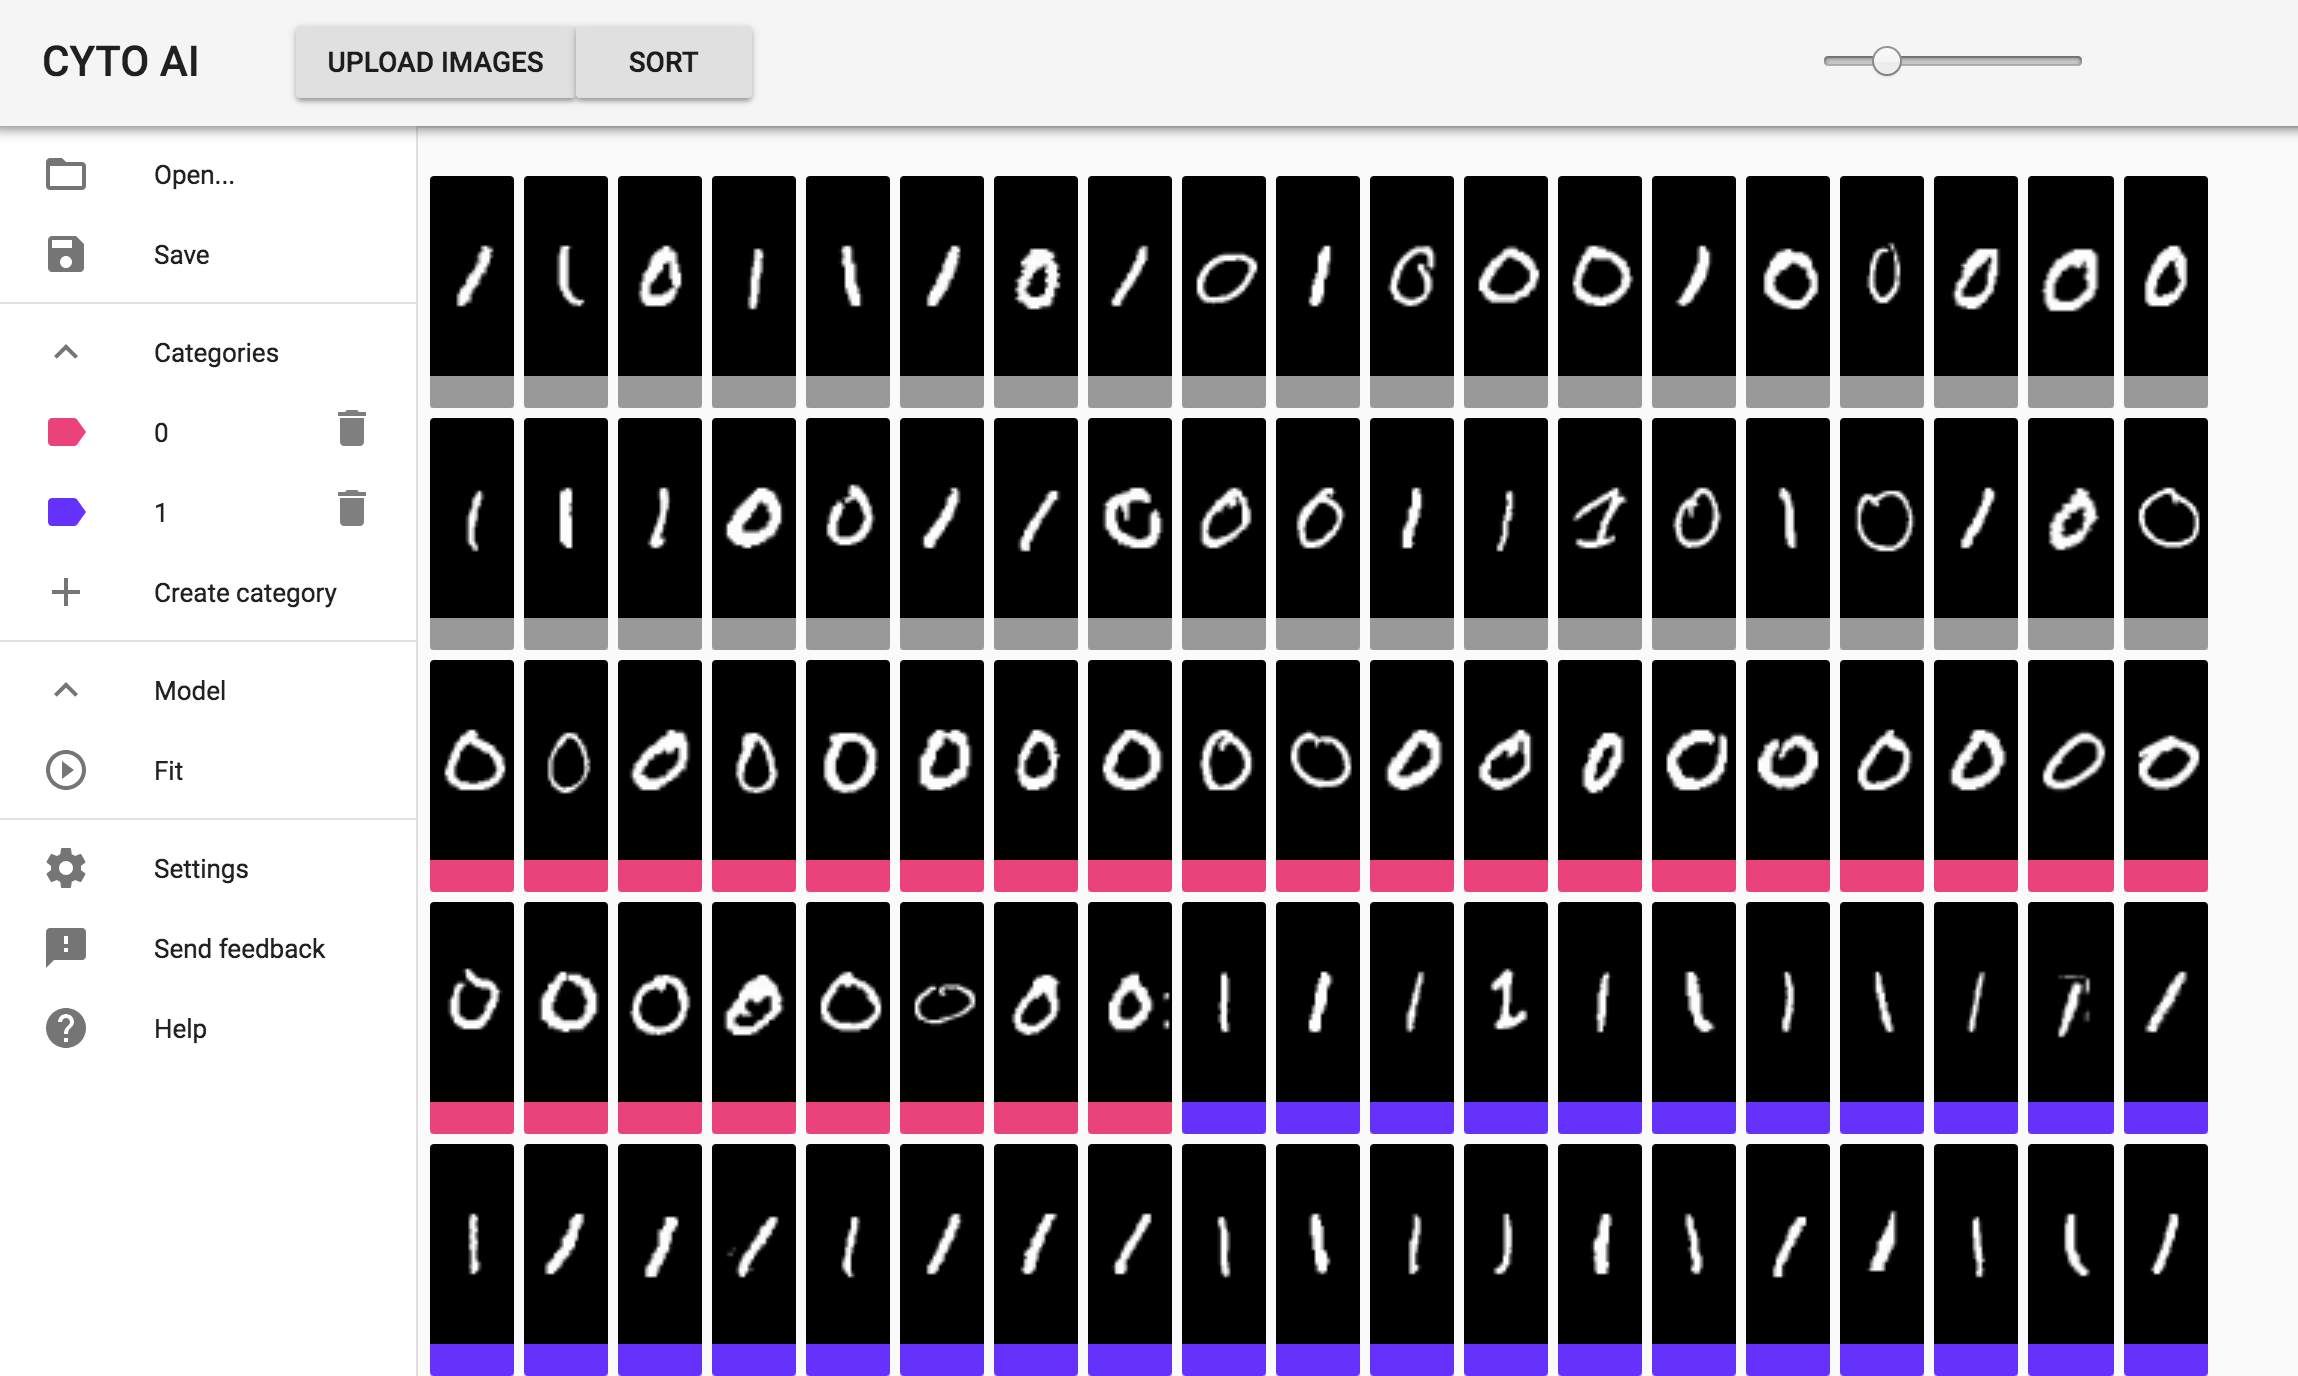
\includegraphics[width=0.8\linewidth]{bilder/cyto/cyto.png}
	\caption{CYOTO AI}
	\label{fig:COMPONENT}
\end{figure}

To save all labels and categories and settings the button can be pressed. To import again the "open" button can be used.


\subsection{System architecture}
The following diagram shall give an overview of how responsibilities are distributed over the system.

\begin{forest}
	for tree={
		font=\ttfamily,
		grow'=0,
		child anchor=west,
		parent anchor=south,
		anchor=west,
		calign=first,
		inner xsep=7pt,
		edge path={
			\noexpand\path [draw, \forestoption{edge}]
			(!u.south west) +(7.5pt,0) |- (.child anchor) pic {folder} \forestoption{edge label};
		},
		% style for your file node 
		file/.style={edge path={\noexpand\path [draw, \forestoption{edge}]
				(!u.south west) +(7.5pt,0) |- (.child anchor) \forestoption{edge label};},
			inner xsep=2pt,font=\small\ttfamily
		},
		before typesetting nodes={
			if n=1
			{insert before={[,phantom]}}
			{}
		},
		fit=band,
		before computing xy={l=15pt},
	}
	[CYTO AI
	[config
	]
	[lib
	[Access
	]
	[Plugin
	]
	[file.txt,file
	]
	]
	[templates
	]
	[tests
	]
	]
\end{forest}


API contains all files and functionality needed for the machine learning classifying task. Folder src contains all components, tests and Redux related files. 
In order to explain how this structure works a further component shall be added.

First a new component "CategoryList" is created. CategoryList shall simply show a list of categories. 

\lstinputlisting{code/cyto/categoryList.js}

The data shall be fetched from a variable categories, placed in the Redux store. In order to fetch this data the component shall be connected to the Redux store so a High-Order Component CategoryListConnector is created. High-Order components wrap a component and add some functionalities in this case it adds the possibility to access the categories array in Redux store. 

\lstinputlisting[caption=CategoryList component]{code/cyto/connectedCategory.js}

The directory will now look like this:

\begin{forest}
	for tree={
		font=\ttfamily,
		grow'=0,
		child anchor=west,
		parent anchor=south,
		anchor=west,
		calign=first,
		inner xsep=7pt,
		edge path={
			\noexpand\path [draw, \forestoption{edge}]
			(!u.south west) +(7.5pt,0) |- (.child anchor) pic {folder} \forestoption{edge label};
		},
		% style for your file node 
		file/.style={edge path={\noexpand\path [draw, \forestoption{edge}]
				(!u.south west) +(7.5pt,0) |- (.child anchor) \forestoption{edge label};},
			inner xsep=2pt,font=\small\ttfamily
		},
		before typesetting nodes={
			if n=1
			{insert before={[,phantom]}}
			{}
		},
		fit=band,
		before computing xy={l=15pt},
	}  
	[system
	[config
	]
	[lib
	[Access
	]
	[Plugin
	]
	[file.txt,file
	]
	]
	[templates
	]
	[tests
	]
	]
\end{forest}


Further it shall be possible to add another category to the category list, therefore an action is needed that takes the new category name and the category color as a payload.

\lstinputlisting[caption=Actions for changing categories]{code/cyto/actions.js}

A reducer will now be called given and the action will be passed to it.

\lstinputlisting[Reducer for changing categories]{code/cyto/categoryReducer.js}

The structure will now look like this:

\begin{forest}
	for tree={
		font=\ttfamily,
		grow'=0,
		child anchor=west,
		parent anchor=south,
		anchor=west,
		calign=first,
		inner xsep=7pt,
		edge path={
			\noexpand\path [draw, \forestoption{edge}]
			(!u.south west) +(7.5pt,0) |- (.child anchor) pic {folder} \forestoption{edge label};
		},
		% style for your file node 
		file/.style={edge path={\noexpand\path [draw, \forestoption{edge}]
				(!u.south west) +(7.5pt,0) |- (.child anchor) \forestoption{edge label};},
			inner xsep=2pt,font=\small\ttfamily
		},
		before typesetting nodes={
			if n=1
			{insert before={[,phantom]}}
			{}
		},
		fit=band,
		before computing xy={l=15pt},
	}  
	[system
	[config
	]
	[lib
	[Access
	]
	[Plugin
	]
	[file.txt,file
	]
	]
	[templates
	]
	[tests
	]
	]
\end{forest}

In short for each added component that needs access to the states a connector needs to be created. Actions and reducers also need to be created to change the state, if not already existing.

\subsection{Machine Learning API}
The machine learning API was built with TensorFlow.js. Every time the "fit" button was clicked an asynchronous API call is made. The calls look like following:

\lstinputlisting{code/cyto/classifier.js}

Where dataset is an instance for handling the data. And imageTags are the HTML . The API is using a CNN Network provided over a Content Delivery Network (CDN).
\subsection{Performance}









%\chapter{Summary and Outlook}

As Samuel Buttler used to say: "Brevity is very good where,
where we are and are not understood." So this summary shall be rather brief.

At the start of the project we had a very powerful but
somewhat difficult to install and use classification
 application written in Python with more than 27.000 lines of code. 
It looked like
an almost impossible task to port such significant piece of
work to an entire new architecture and completely new technologies in just a few months.

Now, at the end of this work and in cooperation with some 
highly talented people, it looks like the decision to
 move to the new web centric development paradigm has 
 paid for itself.

All major technological issues could be resolved and there seems to be good reason to believe that continuing this way
would result in less development effort and better user
experience compared to the traditional way of
implementation.

What is still to be done?

Thus far, the tool can classify entire images. A big step forward would be the capability to segment images, 
that is to locate image areas with objects of interest
prior to the classification process. 

However, this would place considerable demands on the tool and would
require another substantial development effort. The user interface would have to be redesigned so that 
images could be annotated.  

Furthermore, it will soon be possible to export models (trained nets) with Tensorflow.js. The declared aim of Goggle is to make this possible in the upcoming versions (current version 0.10). It is conceivable to make the exported models accessible to other users via a web platform. 


% Alle Eintr�ge der BibTeX Datenbank "zitieren"
\nocite{*}
%Literaturverzeichnis
\bibliographystyle{IEEEtran}
% Auswahl der BibTeX Datenbank f�r das Literaturverzeichnis
\bibliography{thesis}
% Einstellen des Bibliography-Stils f�r das 

% Anhang beginnen (Formatierung umschalten)
\appendix
\chapter{Anhang zum Systementwurf}
Allgemeine Beschreibung des Anhangs

\section{Diagramme}
Hier werden Diagramme platziert, die in den Textkapitel zuviel Platz beanspruchen.
\section{Tabellen}
Hier werden Tabellen platziert, die in den Textkapitel zuviel Platz beanspruchen.
\section{Quellcodelistings}
Hier werden Tabllen platziert, die in den Textkapitel zuviel Platz beanspruchen.


% Ausgabe des Wortindex
% idxtotoc Option scheint nicht zu funktionieren
\clearpage
\addcontentsline{toc}{chapter}{Index}
\printindex


\printglossary[style=altlist, title=Stichwortverzeichnis]
\newpage

% Das Abk�rzungsverzeichnis hat den Typ \acronymtype
\printglossary[type=\acronymtype, style=long, title=Abk�rzungsverzeichnis]
\newpage



% Laut Markus Kohm wird \backmatter normal nicht ben�tigt
%\backmatter
\end{document}
